\documentclass[pdf]{beamer}
\usetheme{Copenhagen}
\usepackage{multicol, latexsym, amsmath, amssymb}
\usepackage{smartdiagram}
\usepackage{subcaption}
\usepackage{natbib}
\usepackage{tikz}
\usepackage{xspace}
\usepackage{amsmath}
\usepackage{amssymb}
\usepackage{tikz}
\usepackage{booktabs}
\usepackage[nobeards,saturated]{tikzpeople}
\usepackage{xspace}
\newcommand*{\error}{\ensuremath{\accDis}\xspace}
\newcommand*{\accuracy}{\ensuremath{\acctest}\xspace}

% training 
\newcommand*{\D}{\ensuremath{\mathcal{D}}\xspace}
\newcommand*{\sample}{\ensuremath{\mathbf{x}}\xspace}
\newcommand*{\dimensions}{\ensuremath{d}\xspace}
\newcommand*{\labels}{\ensuremath{\mathbf{y}}\xspace}

\newcommand*{\Dtrain}{\ensuremath{\D_{\text{init} }}\xspace}
\newcommand*{\Dm}{\ensuremath{\mathcal{D}_{\nremovals}}\xspace}
\newcommand*{\Dprime}{\ensuremath{\D\setminus\Dm}\xspace}
\newcommand*{\Dtest}{\ensuremath{\mathcal{D}_{\text{test}}}\xspace}
\newcommand*{\nremovals}{\ensuremath{m}\xspace}
\newcommand*{\ntrain}{\ensuremath{n_{\text{init}}}\xspace}
\newcommand*{\ntest}{\ensuremath{n}_{\text{test}}\xspace}
\newcommand*{\obj}{\ensuremath{L}\xspace}

%
\newcommand*{\UM}{\ensuremath{u}\xspace}
\newcommand*{\ml}{ML\xspace}
\newcommand*{\sgd}{SGD\xspace}
\newcommand*{\w}{\ensuremath{\mathbf{w}}\xspace}
\newcommand*{\wopt}{\ensuremath{\w^{opt}}\xspace}
\newcommand*{\worig}{\ensuremath{\mathbf{w}^{*}}\xspace}
\newcommand*{\employed}{\ensuremath{e}\xspace}
\newcommand*{\wEmployed}{\ensuremath{\w}\xspace}
\newcommand*{\wunlearned}{\ensuremath{\w^\UM}\xspace}
\newcommand*{\wprime}{\ensuremath{\mathbf{w}^{\prime}}\xspace}
% 

\newcommand*{\efficiencyParameter}{\ensuremath{\tau}\xspace}
\newcommand*{\QoA}{\ensuremath{\efficiencyParameter}\xspace}
\newcommand*{\noiseParamter}{\ensuremath{\sigma}\xspace}
\newcommand*{\unlrbatchsize}{\ensuremath{\nremovals^{\prime}}\xspace}
% Guo et al. 
\newcommand*{\noisyobj}{\ensuremath{\obj_{\sigma}}\xspace}
\newcommand*{\infl}{\textsc{Influence}\xspace}
\newcommand*{\guo}{\textsc{guo}\xspace}

% Golatkar et al.
\newcommand*{\fisher}{\textsc{Fisher}\xspace}
\newcommand*{\fMatrix}{\ensuremath{F}\xspace}
\newcommand*{\gol}{\textsc{gol}\xspace}

% Wu et al. 
\newcommand*{\wu}{\textsc{wu}\xspace}
\newcommand*{\deltagrad}{\textsc{DeltaGrad}\xspace}
\newcommand*{\iw}{\ensuremath{\w}\xspace}
\newcommand*{\dgapprox}{\textsc{DGApprox}\xspace}

% Distribution Experiment
\newcommand*{\classprob}{p_{\text{class}}\xspace}
\newcommand*{\infoprob}{p_{\text{info}}\xspace}

% Datasets

\newcommand*{\bmnist}{\ensuremath{\text{\sc mnist}^{\text{b}}}\xspace}
\newcommand*{\mnist}{\text{\sc mnist}\xspace}
\newcommand*{\covtype}{\text{\sc covtype}\xspace}
\newcommand*{\higgs}{\text{\sc higgs}\xspace}
\newcommand*{\cifar}{\text{\sc cifar2}\xspace}
\newcommand*{\eps}{\text{\sc epsilon}\xspace}
\newcommand*{\T}{\top}
\newcommand*{\x}{\mathbf{x}\space}
\newcommand*{\noiseb}{\ensuremath{\mathbf{b}}\xspace}

% metrics
\newcommand{\smape}{\ensuremath{\text{\tt SMAPE}}\xspace}
\newcommand{\sape}{\ensuremath{\text{\tt SAPE}}\xspace}
\newcommand{\acctest}{\ensuremath{\text{\tt Acc}_{\text{test}}}\xspace}
\newcommand{\accremoved}{\ensuremath{\text{\tt Acc}_{\text{del}}}\xspace}
\newcommand*{\accErr}{\texttt{AccErr}\xspace}
\newcommand*{\accDrop}{\accErr}
\newcommand*{\relEff}{\accDrop}
\newcommand*{\accDis}{\texttt{AccDis}\xspace}

% sampling types 

\newcommand{\unirand}{\text{{\tt uniform-random}}\xspace}
\newcommand{\targrand}{\text{{\tt targeted-random}}\xspace}
\newcommand{\uniinfo}{\text{{\tt uniform-informed}}\xspace}
\newcommand{\targinfo}{\text{{\tt targeted-informed}}\xspace}

% When to retrain
\newcommand*{\winit}{\ensuremath{\worig_{\text{init}}}\xspace}
\newcommand*{\accdropinit}{\ensuremath{\accDrop_{\text{init}}}\xspace}
\newcommand*{\acctestinit}{\ensuremath{\acctest^{\text{init}}}\xspace}
\newcommand*{\slope}{\ensuremath{c}\xspace}
\newcommand*{\disPred}{\ensuremath{\overline{\error}}\xspace}
\newcommand*{\estErr}{\ensuremath{EstErr}\xspace}
\newcommand*{\estDis}{\ensuremath{EstDis}\xspace}
\newcommand*{\thresh}{\ensuremath{\kappa}\xspace}

%
\newcommand*{\repo}{\url{https://version.helsinki.fi/mahadeva/unlearning-experiments}}

\newcommand*{\good}{\ensuremath{\uparrow}}
\newcommand*{\better}{\ensuremath{\uparrow\uparrow}}
\newcommand*{\best}{\ensuremath{\uparrow\uparrow\uparrow}}
\newcommand{\revision}[1]{\textcolor{blue}{{#1}}}

\newcommand*{\inc}{\ensuremath{\textcolor{green!80!black}\uparrow}}
\newcommand*{\dec}{\ensuremath{\textcolor{red!80!black}\downarrow}}






% Allow local line spacing changes
\usepackage{setspace}
\usepackage{xcolor}
\usepackage[export]{adjustbox}
\usepackage{pifont}
\usepackage{bbding}
\usepackage[nobeards,saturated]{tikzpeople}
\usetikzlibrary{positioning,arrows,shapes.misc,shapes.geometric,decorations.markings}
\definecolor{antiquewhite}{rgb}{0.98, 0.92, 0.84}
\definecolor{beige}{rgb}{0.96, 0.96, 0.86}
\definecolor{blond}{rgb}{0.98, 0.94, 0.75}
\tikzset{blackbox/.style={shirt=black,hair=black}}
\tikzset{whitebox/.style={shirt=blond,hair=blond}}
\tikzset{graybox/.style={shirt=gray,hair=gray}}
\newcommand{\adv}{\ensuremath{\mathcal{A}}\xspace}


% algorithms
\newcommand{\opt}{\textsc{OPT}\xspace}
\newcommand{\wmsketch}{\textsc{WM-Sketch}\xspace}
\newcommand{\wmsketches}{\textsc{WM-Sketch}es\xspace}
\newcommand{\learner}{\textsc{Learner}\xspace}
\newcommand{\adversary}{\textsc{Adversary}\xspace}
\newcommand{\countsketch}{count sketch\xspace}
% datasets
% \newcommand{\mnist}{\textsc{MNIST}\xspace}

% Global SGD-related
\newcommand{\featureset}{\ensuremath{\mathcal{X}}\xspace}
\newcommand{\featuresetbound}{\ensuremath{\gamma}\xspace}
\newcommand{\nfeats}{\ensuremath{d}\xspace}
\newcommand{\labelset}{\ensuremath{\mathcal{Y}}\xspace}
\newcommand{\history}{\ensuremath{\mathcal{H}}\xspace}
% \newcommand{\x}{\ensuremath{\mathbf{x}}\xspace}
\newcommand{\xt}[1]{\ensuremath{\mathbf{x}^{#1}}\xspace}
\newcommand{\y}{\ensuremath{y}\xspace}
\newcommand{\yt}[1]{\ensuremath{y^{#1}}\xspace}
\newcommand{\modelerror}{\ensuremath{\epsilon}\xspace}
\newcommand{\lr}{\ensuremath{\eta^{t}}\xspace}
\newcommand{\querybudget}{\ensuremath{T}\xspace}
\newcommand{\plainloss}[1]{\ensuremath{l\round{#1}}\xspace}
\newcommand{\loss}[1]{\ensuremath{l\round{#1}}\xspace}
\newcommand{\projsgd}{\ensuremath{\texttt{Proj}}\xspace}
\newcommand{\predict}[1]{\ensuremath{\text{sign}\round{\product{#1}}}\xspace}

% uncompressed classifier
% \newcommand{\w}{\ensuremath{\textbf{w}}\xspace}
\newcommand{\wt}[1]{\ensuremath{\w^{#1}}\xspace}
\newcommand{\wstar}{\wt{*}\xspace}
\newcommand{\woptgap}[1]{\w{#1} - \wstar}
\newcommand{\hypspace}{\ensuremath{\mathcal{W}}\xspace}
\newcommand{\hypspacebound}{\ensuremath{D}\xspace}
\newcommand{\yhatuc}{\ensuremath{\hat{\y}}\xspace}
\newcommand{\ythatuc}[1]{\ensuremath{\hat{\y}^{#1}}\xspace}

% sketched classifier
\newcommand{\z}{\ensuremath{\textbf{z}}\xspace}
\newcommand{\zt}[1]{\ensuremath{\z^{#1}}\xspace}
\newcommand{\zstar}{\zt{*}\xspace}
\newcommand{\zoptgap}[1]{\z{#1} - \zstar}
\newcommand{\hypspacec}{\ensuremath{\mathcal{Z}}\xspace}
\newcommand{\JLmat}{\ensuremath{R}\xspace}
\newcommand{\yhatc}{\ensuremath{\hat{\y}_{\textsc{WM}}}\xspace}
\newcommand{\ythatwr}[1]{\ensuremath{\hat{\y}^{#1}_{\text{WR}}}\xspace}
\newcommand{\ythatfp}[1]{\ensuremath{\hat{\y}^{#1}_{\text{FP}}}\xspace}
\newcommand{\sketchsize}{\ensuremath{k}\xspace}
\newcommand{\sketchdepth}{\ensuremath{s}\xspace}
\newcommand{\hfh}{\ensuremath{h}\xspace}
\newcommand{\hfsigma}{\ensuremath{\sigma}\xspace}
\newcommand{\west}{\ensuremath{\hat{\w}_{\textsc{WM}}}\xspace}
\newcommand{\westt}[1]{\ensuremath{\hat{\w}^{#1}_{\textsc{WM}}}\xspace}
\newcommand{\globalscale}{\ensuremath{\alpha}\xspace}

% attack model
\newcommand{\mislead}{\textsc{l}\xspace}
\newcommand{\misclassify}{\textsc{c}\xspace}
\newcommand{\whitebox}{\textsc{wb}\xspace}
\newcommand{\greybox}{\textsc{gb}\xspace}
\newcommand{\blackbox}{\textsc{bb}\xspace}
\newcommand{\direct}{\textsc{d}\xspace}
\newcommand{\transfers}{\textsc{st}\xspace}
\newcommand{\transferl}{\textsc{lt}\xspace}
\newcommand{\WBD}{\whitebox-\direct}
\newcommand{\GBTS}{\greybox-\transfers}
\newcommand{\BBTL}{\blackbox-\transferl}
\newcommand{\perturb}{\ensuremath{\delta}\xspace}
\newcommand{\xtilde}[1]{\ensuremath{\tilde{\mathbf{x}}^{#1}}\xspace}

\definecolor{forestgreen}{rgb}{0.13, 0.55, 0.13}
\newcommand*{\tick}{\textcolor{forestgreen}{\textnormal{\Checkmark}}}
\newcommand*{\cross}{\textcolor{red}{\textnormal{\XSolidBold}}}

\newcommand{\cmark}{\textcolor{green!80!black}{\ding{51}}}
\newcommand{\xmark}{\textcolor{red}{\ding{55}}}


% \newcommand*{\ml}{ML}

\newcommand*{\decision}{\ensuremath{\mathcal{R}}\xspace}
% \newcommand*{\QDM}{\ensuremath{\text{\sc QDM}}\xspace}
\newcommand*{\QDMq}{\ensuremath{\psi}\xspace}
\newcommand*{\QDM}{\ensuremath{\Psi}\xspace}
% \newcommand*{\QDMdiff}{\ensuremath{\QDM_{\text{diff}}}\xspace}
\newcommand*{\QDMdiff}{\ensuremath{\overline{\Psi}}\xspace}
\newcommand*{\simfn}{\ensuremath{\text{sim}}\xspace}
% \newcommand*{\loss}{\ensuremath{\ell}\xspace}
\newcommand*{\tprime}{\ensuremath{t^{\prime}}\xspace}
\newcommand*{\feat}{\ensuremath{d}\xspace}
\newcommand*{\q}{\ensuremath{q}\xspace}
% \newcommand*{\x}{\ensuremath{x}\xspace}
% \newcommand*{\y}{\ensuremath{y}\xspace}
\newcommand*{\X}{\ensuremath{\mathbf{X}}\xspace}
\newcommand*{\Y}{\ensuremath{\mathbf{y}}\xspace}
\newcommand*{\Yset}{\ensuremath{\mathcal{Y}}\xspace}
\newcommand*{\Xset}{\ensuremath{\mathcal{X}}\xspace}
\newcommand*{\ttime}{\ensuremath{t}\xspace}
\newcommand*{\data}{\ensuremath{D}\xspace}
\newcommand*{\model}{\ensuremath{M}\xspace}
\newcommand*{\query}{\ensuremath{Q}\xspace}
\newcommand*{\Dtprime}{\ensuremath{\data_{\tprime}}\xspace}
\newcommand*{\Mtprime}{\ensuremath{\model_{\tprime}}\xspace}
\newcommand*{\Qtprime}{\ensuremath{\query_{\tprime}}\xspace}
\newcommand*{\Dt}{\ensuremath{\data_{t}}\xspace}
\newcommand*{\Mt}{\ensuremath{\model_{t}}\xspace}
\newcommand*{\Qt}{\ensuremath{\query_{t}}\xspace}
\newcommand*{\dataBatch}{\ensuremath{B_\data}\xspace}
\newcommand*{\queryBatch}{\ensuremath{B_\query}\xspace}
% \newcommand*{\T}{\ensuremath{T}\xspace}
\newcommand*{\offline}{\text{offline}\xspace}
\newcommand*{\online}{\text{online}\xspace}
\newcommand*{\Toffline}{\ensuremath{\T_{\offline}}\xspace}
\newcommand*{\Tonline}{\ensuremath{\T_{\online}}\xspace}
\newcommand*{\Tstart}{\ensuremath{\T_{\text{start}}}\xspace}
\newcommand*{\Tend}{\ensuremath{\T_{\text{end}}}\xspace}
\newcommand*{\Cost}{\ensuremath{C}\xspace}
\newcommand*{\totalcost}{\ensuremath{c}\xspace}
\newcommand*{\cost}[1]{\ensuremath{\text{cost}\round{#1}}\xspace}
\newcommand*{\dpcost}[2][]{%
    \ifx\\#1\\%
        \ensuremath{v\round{#2}}\xspace%
        \else%
        \ensuremath{v^{#1}\round{#2}}\xspace%
    \fi%
}
\newcommand*{\prev}{\ensuremath{p}\xspace}
\newcommand*{\dptable}{\ensuremath{V}\xspace}
\newcommand*{\costmatrix}{\Cost}
\newcommand*{\costentry}[1]{\ensuremath{c_{#1}}\xspace}
\newcommand*{\strategy}{\ensuremath{S}\xspace}
\newcommand*{\partialstrategy}{\ensuremath{\bar{\strategy}}\xspace}
\newcommand*{\partialstrategyopt}{\ensuremath{\round{\partialstrategy}^{*}}\xspace}

\newcommand*{\oracleretrains}{\ensuremath{O}\xspace}
\newcommand*{\retraincost}{\ensuremath{\kappa}\xspace}

\newcommand*{\retrain}{\texttt{Retrain}\xspace}
\newcommand*{\keep}{\texttt{Keep}\xspace}


%algorithms

\newcommand*{\oracle}{\textsc{Oracle}\xspace}
\newcommand*{\neverretrain}{\textsc{NR}\xspace}
\newcommand*{\algo}{\textsc{Cara}\xspace}
\newcommand*{\cara}{\algo}
\newcommand*{\algoparams}{\ensuremath{\theta}\xspace}
\newcommand*{\algoparamsopt}{\ensuremath{\algoparams^{*}}\xspace}

\newcommand*{\markov}{\textsc{Markov}\xspace}
\newcommand*{\algoMarkov}{\textsc{\algo-M}\xspace}
\newcommand*{\algoThresh}{\textsc{\algo-T}\xspace}
% \newcommand*{\thresh}{\ensuremath{\tau}\xspace}
\newcommand*{\threshopt}{\ensuremath{\thresh^{*}}\xspace}
\newcommand*{\cumthresh}{\ensuremath{\tau_\text{cum}}\xspace}
\newcommand*{\cumthreshopt}{\ensuremath{\cumthresh^{*}}\xspace}

\newcommand*{\algoCummThresh}{\textsc{\algo-CT}\xspace}
\newcommand*{\algoPeriod}{\textsc{\algo-P}\xspace}
\newcommand*{\period}{\ensuremath{\phi}\xspace}
\newcommand*{\periodopt}{\ensuremath{\period^{*}}\xspace}
\newcommand*{\offset}{\ensuremath{a}\xspace}
\newcommand*{\offsetopt}{\ensuremath{\offset^{*}}\xspace}


%baselines
\newcommand*{\adwin}{\textsc{ADWIN}\xspace}
\newcommand*{\ddm}{\textsc{DDM}\xspace}

%metrics 
\newcommand*{\scpe}{\texttt{SCPE}\xspace}
%datasets
\newcommand*{\covcon}{\textsc{CovCon}\xspace}
\newcommand*{\covconData}{\textsc{\covcon-D}\xspace}
\newcommand*{\covconStatic}{\textsc{\covcon-S}\xspace}
\newcommand*{\Circle}{\textsc{Circle}\xspace}
\newcommand*{\Circles}{\Circle}
\newcommand*{\circles}{\Circle}
\newcommand*{\circlesData}{\textsc{\Circle-D}\xspace}
\newcommand*{\circlesStatic}{\textsc{\Circle-S}\xspace}
\newcommand*{\gauss}{\textsc{Gauss}\xspace}
\newcommand*{\gaussData}{\textsc{\gauss-D}\xspace}
\newcommand*{\gaussStatic}{\textsc{\gauss-S}\xspace}
\newcommand*{\elec}{\textsc{Electricity}\xspace}
\newcommand*{\covertype}{\textsc{Covertype}\xspace}
% \newcommand*{\covtype}{\textsc{Covtype}\xspace}
\newcommand*{\airlines}{\textsc{Airlines}\xspace}
\newcommand*{\fixedretraincost}{\ensuremath{46}}


\setbeamercovered{transparent}
\beamertemplatenavigationsymbolsempty
\setbeamertemplate{footline}[text line]{%
    \parbox{\linewidth}{\vspace*{-8pt}\hfill\hfill\insertframenumber\,/\,\inserttotalframenumber}}
% \setbeamertemplate{navigation symbols}{}
% \newcommand{\z}{\mathbf{z}}
\newcommand{\uout}{u_{out}}
\newcommand{\vout}{v_{out}}
\newcommand{\uoutdum}{u_{out}^{dum}}
\newcommand{\uinplus}{u_{in}^{+}}
\newcommand{\uinminus}{u_{in}^{-}}
\newcommand{\winl}{w_{in}^{l}}
\newcommand{\win}{w_{in}}
\newcommand{\uin}{w_{in}}
\newcommand{\vin}{v_{in}}

\DeclareMathOperator*{\plusrightarrow}{\ensuremath{\xrightarrow{+}}}
\DeclareMathOperator*{\minusrightarrow}{\ensuremath{\xrightarrow{-}}}
\DeclareMathOperator*{\plusleftarrow}{\ensuremath{\xleftarrow{+}}}
\DeclareMathOperator*{\minusleftarrow}{\ensuremath{\xleftarrow{-}}}

\title{Thesis Committee Meeting}

\author[Ananth Mahadevan]{Ananth Mahadevan}
\date{\today}

\begin{document}
\begin{frame}
    \titlepage
\end{frame}

\begin{frame}
    \frametitle{Overview}
    \tableofcontents
\end{frame}

\section{Research}

\subsection{Published Articles}
\begin{frame}<1>[label=published]
    \frametitle{Published Articles}
    \begin{enumerate}[<+->]
        \item Certifiable Unlearning for logistic regression: An experimental study, MAKE 2022 \cite{mahadevan2022certifiable}
        \item Scalably Using Node Attributes and Graph Structure for Node Classification, Entropy 2022 \cite{merchant2022JANE}
        \item Robustness of Sketched Linear Classifiers to Adversarial Attacks, CIKM 2022 \cite{10.1145/3511808.3557687}
        \item Reception Reader: Exploring Text Reuse in Early Modern British Publications, JOHD 2023 \cite{Rosson-2023}
    \end{enumerate}
\end{frame}


\begin{frame}
    \frametitle{Machine Unlearning }
    \scalebox{0.5}{
    \begin{tikzpicture}
        \newcommand\file[2]{%
    \begin{scope}[xshift=#1cm,yshift=#2cm]
      \draw[gray,thick] (0,0) -- (0,1.5) -- (0.7,1.5) -- (0.7,1.1) -- (1,1.1) -- (1,0) -- cycle;
      \draw[gray,thick] (0.7,1.5) -- (1,1.1);
      \foreach \y in {0.2,0.3,...,1.1}{
         \draw[thick] (0.2,\y) -- (0.8,\y);
         }
      \foreach \y in {1.1,1.2,...,1.4}{
         \draw[thick] (0.2,\y) -- (0.65,\y);
         }
        %  \draw[thick] (0.2,0.8) -- (0.6,0.8);
        %  \draw[thick] (0.2,1) -- (0.6,1);
    \end{scope}
}

% https://tex.stackexchange.com/questions/126161/how-can-i-draw-a-tikz-element-multiple-times-against-a-shaded-background
% \pgfkeys{/tikz/.cd,
%    at/.initial={(0,0)},
%    at/.get=\coordpos,
%    at/.store in=\coordpos,   
%    my tree/.code={
%     \draw[gray] \coordpos -- +(0,1.2) -- +(0.7,1.2) -- +(0.7,0.8) -- +(1,0.8) -- +(1,0) -- cycle;
%     \draw[gray] +(0.7,1.2) -- +(1,0.8);
%     \foreach \y in {0.2,0.4,0.6}{
%         \draw (0.2,\y) -- (0.8,\y);
%         \draw (0.2,0.8) -- (0.6,0.8);
%         \draw (0.2,1) -- (0.6,1);
%     }
%    }
% }
\begin{tikzpicture}
    \tikzset{
      piece/.style 2 args={red,draw,thick,rectangle,anchor=south west,minimum width=#1,minimum height=#2},
      defrag piece/.style 2 args={blue,draw,thick,rectangle,anchor=south west,minimum width=#1,minimum height=#2},
      source piece/.style 2 args={orange,draw,very thick,rectangle,anchor=south west,minimum width=#1,minimum height=#2},
      destination piece/.style 2 args={green!50!black,draw,very thick,rectangle,anchor=south west,minimum width=#1,minimum height=#2},
      reuse/.style={red,-,very thick},
      defrag reuse/.style={blue,-,very thick},
      reception/.style={black,-{Latex[scale=1]},very thick},
    %   cluster/.style={violet,-,very thick}
    cluster/.style={violet,-,very thick,rounded corners=10pt,rectangle},
    }
    \begin{scope}[local bounding box=scope1]
    % \draw [help lines] (0,-2) grid (4,4);
    \file{0}{0}
    \node at (0.5,1.65) {A};
    \node[piece={0.8cm}{0.4cm}] at (0.1,0.1) (tr11) {};
    \node[piece={0.54cm}{0.4cm}] at (0.1,1.1) (tr12) {};
    \file{1.5}{1.5}
    \node at (2,3.15) {B};
    \node[piece={0.8cm}{0.4cm}] at (1.55,1.55) (tr21) {};
    \node[piece={0.78cm}{0.5cm}] at (1.64,1.63) (tr22) {};
    \file{3}{0}
    \node at (3.5,1.65) {C};
    \node[piece={0.54cm}{0.4cm}] at (3.1,0.95) (tr31) {};
    \node[piece={0.8cm}{0.4cm}] at (3.1,0.1) (tr32) {};
    \file{1.5}{-1.5}
    \node at (2,0.15) {D};
    \node[piece={0.8cm}{0.4cm}] at (1.55,-1.45) (tr41) {};
    \node[piece={0.78cm}{0.5cm}] at (1.63,-1.36) (tr42) {};
    \draw[reuse] (tr12.east) -- (tr21.west);
    \draw[reuse] (tr11.east) -- (tr41.west);
    \draw[reuse] (tr42.east) -- (tr32.west);
    \draw[reuse] (tr22.east) -- (tr31.west);
    % \node at (2,-1.68) {};
    % \matrix [below left] at (current bounding box.north east) {
    % \node [piece={0.5cm}{0.1cm},label=right:Piece] {};\\
    % \node[reuse,inner sep=0,minimum width=4mm,draw,anchor= south west,label=right:Text Reuse] at ++(1mm,0) {};\\
    % };
    \end{scope}
    \uncover<2->{
    \begin{scope}[local bounding box=scope2,shift={(scope1.base east)},xshift=3cm]
    % \draw [help lines] (0,-2) grid (4,4);
    \file{0}{0}
    \node at (0.5,1.65) {A};
    \node[defrag piece={0.8cm}{0.4cm}] at (0.1,0.1) (tr11) {};
    \node[defrag piece={0.54cm}{0.4cm}] at (0.1,1.1) (tr12) {};
    \file{1.5}{1.5}
    \node at (2,3.15) {B};
    \node[defrag piece={0.8cm}{0.54cm}] at (1.58,1.6) (tr21) {};
    \file{3}{0}
    \node at (3.5,1.65) {C};
    \node[defrag piece={0.54cm}{0.4cm}] at (3.1,0.95) (tr31) {};
    \node[defrag piece={0.8cm}{0.4cm}] at (3.1,0.1) (tr32) {};
    \file{1.5}{-1.5}
    \node at (2,0.15) {D};
    \node[defrag piece={0.8cm}{0.54cm}] at (1.6,-1.4) (tr41) {};
    \draw[defrag reuse] (tr12.east) -- (tr21.west);
    \draw[defrag reuse] (tr11.east) -- (tr41.west);
    \draw[defrag reuse] (tr41.east) -- (tr32.west);
    \draw[defrag reuse] (tr21.east) -- (tr31.west);
    
    % \draw[cluster] plot [smooth cycle] coordinates{(0.1,1) (3.8,0.95) (3.5,2) (2,2.25) (0.6,2) };
    % \draw[cluster] plot [smooth cycle] coordinates{(0.0,0.6)  (4,0.6) (3.5,-1) (2,-1.75) (0.55,-1)};
    \uncover<3->{
    \draw[cluster] (-0.1,0.9) rectangle (4,2.3) ;
    \draw[cluster] (-0.1,0.6) rectangle (4,-1.5) ;
    }
    \end{scope}
    \draw [->,black,very thick] ($(scope1.east)!0.1!(scope2.west)$) -- ($(scope1.east)!0.9!(scope2.west)$) node[midway,above,align=center]{Defragment} node[midway,below] {\only<3->{\& Cluster}};
    }
    \uncover<4->{
    \begin{scope}[local bounding box=scope3,shift={(scope2.base east)},xshift=3cm]
      % \draw [help lines] (0,-2) grid (4,4);
      \file{0}{0}
      \node at (0.5,1.65) {A};
      \node[source piece={0.8cm}{0.4cm}] at (0.1,0.1) (tr11) {};
      \node[alt=<-4>{defrag piece={0.54cm}{0.4cm}}{destination piece={0.54cm}{0.4cm}}] at (0.1,1.1) (tr12) {};
      \file{1.5}{1.5}
      \node at (2,3.15) {B};
      \node[source piece={0.8cm}{0.54cm}] at (1.58,1.6) (tr21) {};
      \file{3}{0}
      \node at (3.5,1.65) {C};
      \node[alt=<-4>{defrag piece={0.54cm}{0.4cm}}{destination piece={0.54cm}{0.4cm}}] at (3.1,0.95) (tr31) {};
      \node[alt=<-4>{defrag piece={0.8cm}{0.4cm}}{destination piece={0.8cm}{0.4cm}}] at (3.1,0.1) (tr32) {};
      \file{1.5}{-1.5}
      \node at (2,0.15) {D};
      \node[alt=<-4>{defrag piece={0.8cm}{0.54cm}}{destination piece={0.8cm}{0.54cm}}] at (1.6,-1.4) (tr41) {};
      \uncover<6->{
      \draw[reception] (tr11.east) -- (tr41.west);
      \draw[reception] (tr11.east) -- (tr32.west);

      \draw[reception] (tr21.west) -- (tr12.east);
      \draw[reception] (tr21.east) -- (tr31.west);
      }
    %   \draw[cluster] plot [smooth cycle] coordinates{(0.1,1) (3.8,0.95) (3.5,2) (2,2.25) (0.6,2) };
    %   \draw[cluster] plot [smooth cycle] coordinates{(0.0,0.6)  (4,0.6) (3.5,-1) (2,-1.75) (0.55,-1)};
    \draw[cluster] (-0.1,0.9) rectangle (4,2.3) ;
    \draw[cluster] (-0.1,0.6) rectangle (4,-1.5) ;
      \end{scope}
      
      
      \draw [->,black,very thick] ($(scope2.east)!0.1!(scope3.west)$) -- ($(scope2.east)!0.9!(scope3.west)$) node[midway,above]{Identify Source}  node[midway,below] {\only<5->{\& Destinations}};
      
    }
    \matrix [draw,matrix anchor = south,yshift=5mm] at (current bounding box.north)
    % ($(scope1.north west)!0.5!(scope3.north east)$) 
    {
    \node [piece={0.5cm}{0.1cm},label=right:Piece] {}; & 
      \node [defrag piece={0.5cm}{0.1cm},label=right:Defrag Piece] {}; &
      \node [source piece={0.5cm}{0.1cm},label=right:Src Piece] {}; &
      \node[draw,cluster,anchor=south west,minimum width=0.5cm,minimum height=0.1cm,rounded corners=2pt,rectangle,label=right:Cluster] {};\\
    %   \node [destination piece={0.5cm}{0.1cm},label=right:Destination Piece] {}; &\\
      \node[reuse,inner sep=0,minimum width=4mm,draw,anchor=south west,label=right:Reuse] at ++(0,1mm) {}; &
      \node[defrag reuse,inner sep=0,minimum width=4mm,draw,anchor= south west,label=right:Defrag Reuse] at ++(0,1mm) {}; &
      \node [destination piece={0.5cm}{0.1cm},label=right:Dest Piece] {}; &
      \draw[reception] (0,1mm) -- (5mm,1mm) node[inner sep =0,minimum size =0,right,anchor=west] {Reception};
      \node [inner sep=0,label=right:Doc,anchor=south west] at (2.2cm,-0.5mm){\faFileTextO};&
    \\
    };
\end{tikzpicture}
      \end{tikzpicture}
    }

    \begin{block}{Unlearning}
        Task of updating a ML model after partial deletion of training data
    \end{block}
    Qualities of an approximate unlearning method:
  \begin{itemize}
    \item \textbf{Certifiability}: How similar are \wunlearned and \worig?
    \item \textbf{Effectiveness}: How well does \wunlearned perform?
    \item \textbf{Efficiency}: How much time to produce \wunlearned?
  \end{itemize}

\end{frame}

\begin{frame}
    \frametitle{Experimental Setup}
    \begin{center}
        \begin{tabular}{cc}
          \toprule
          Item & Values  \\
          \midrule
          Parameters & Noise (\noiseParamter) \& Efficiency (\efficiencyParameter)  \\
          Metrics & \accDis, \accErr \& Speedup(\texttimes) \\
          Methods & \textcolor{blue!80!black}{\infl}, \textcolor{orange!90!black}{\fisher} \& \textcolor{green!60!black}{\deltagrad}\\
          \bottomrule
        \end{tabular}
      \end{center}
      \begin{center}
        \begin{tabular}{cc}
          \toprule
          Metric & Quality \\
          \midrule
          \accDis\inc & Certifiability\dec\\
          \accErr\inc & Effectiveness\dec\\
          \bottomrule
        \end{tabular}
    \end{center}
        \begin{center}
            \begin{tabular}{cc}
              \toprule
              Parameter & Effect\\
              \midrule
              $\efficiencyParameter\inc$ & $\text{Efficiency}\inc\text{ Certifiability}\dec\text{ Effectiveness}\dec$\\
              $\noiseParamter\inc$ & $\text{Certifiability}\inc\text{ Effectiveness}\dec$\\ 
              \bottomrule
            \end{tabular}
        \end{center}
                

\end{frame}

% \begin{frame}
%     \frametitle{Results}
%     \begin{columns}
%         \begin{column}{0.5\textwidth}
%             \begin{center}
%                 {\small Varying $\tau$}\\
%                 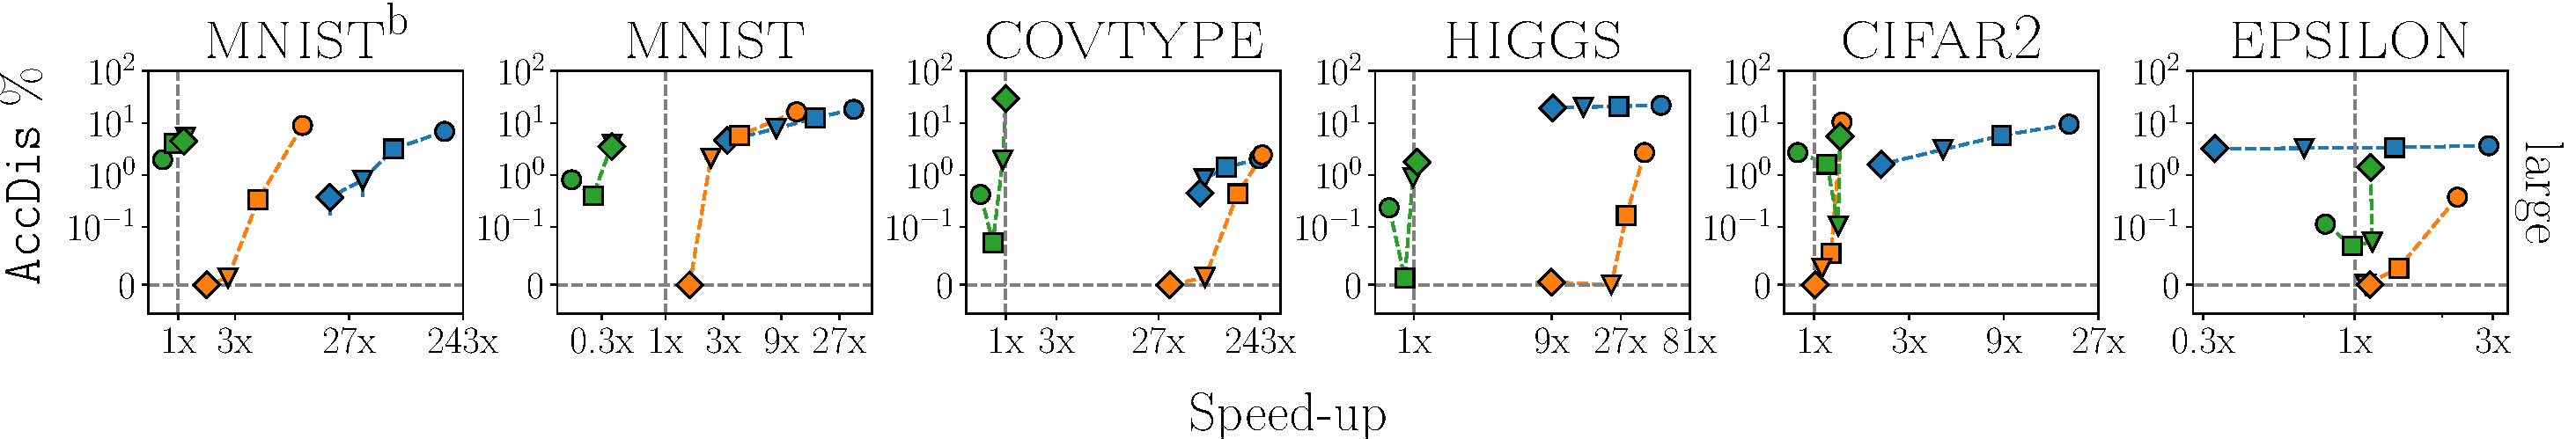
\includegraphics[width=0.6\linewidth,trim={0 1cm 39cm 0},clip]{figs/Certifiability_Efficiency_Trade_Off_Grid_large_sigma_1.pdf}\\
%                 (a) Certifiability
%                 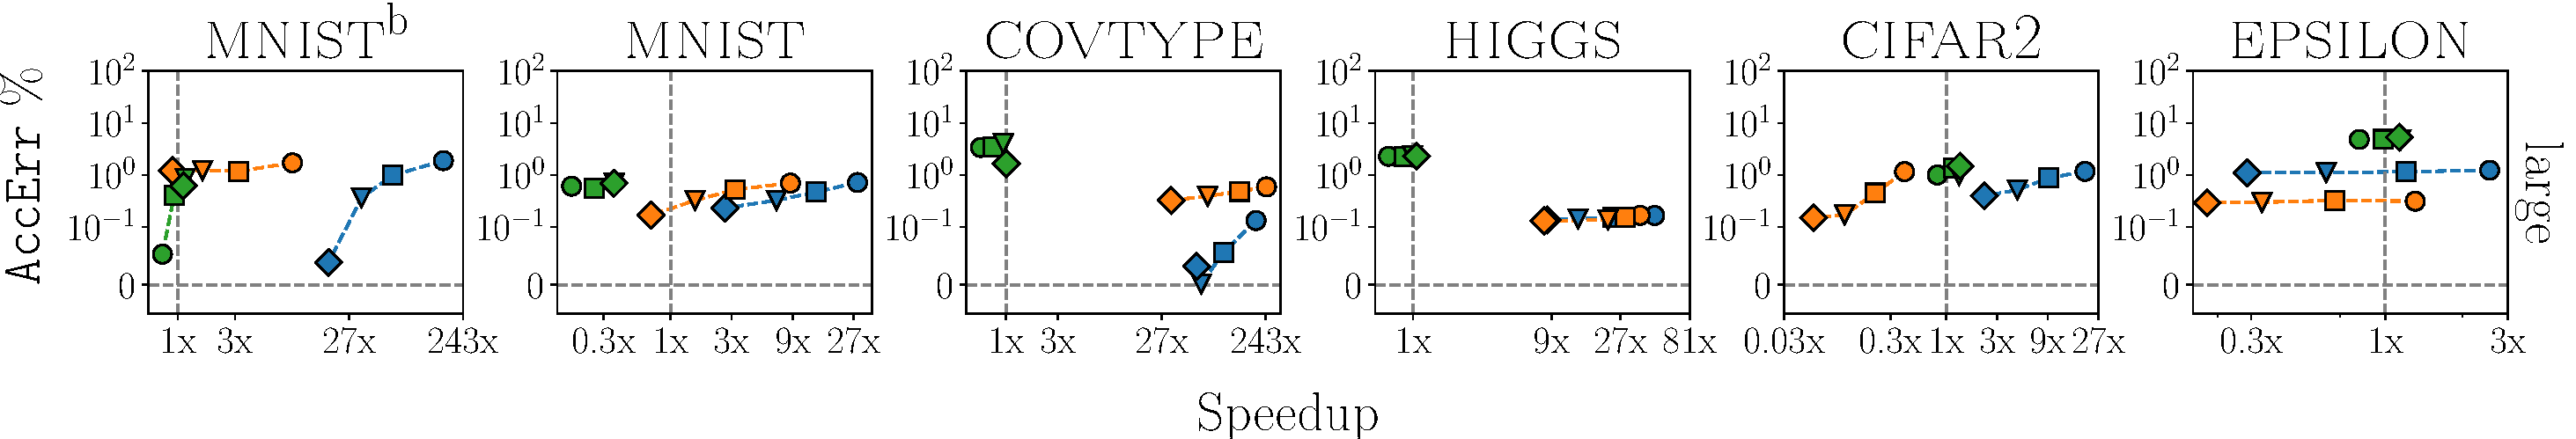
\includegraphics[width=0.6\linewidth,trim={0 1cm 39cm 0},clip]{figs/Effectiveness_Efficiency_Trade_Off_Grid_large_sigma_1.pdf}\\
%                 (b) Effectiveness  
%                 \end{center}        
%         \end{column}
%         \begin{column}{0.5\textwidth}
%             \begin{center}
%                 {\small Varying $\sigma$}\\
%                 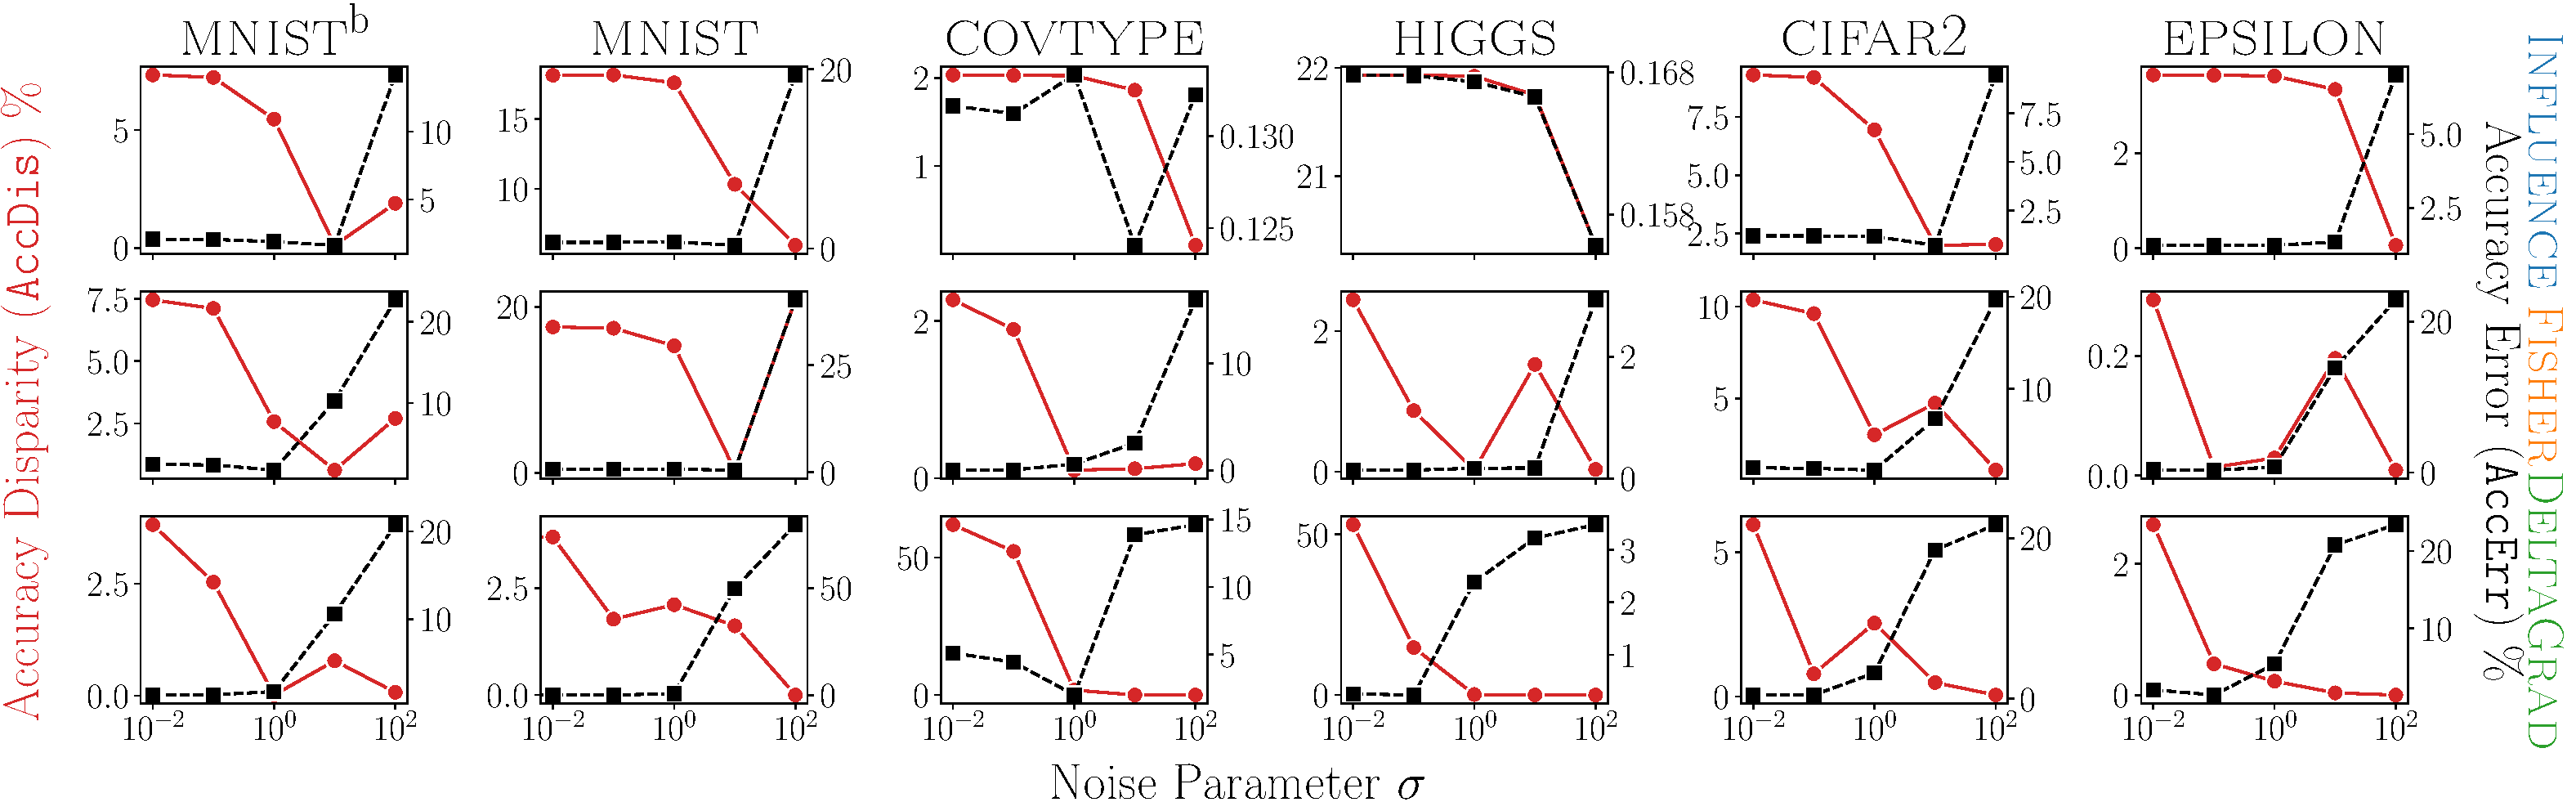
\includegraphics[width=0.08\linewidth,clip,trim={0 1cm 52cm 1.52cm }]{./figs/Unlearning_Tradeoff_Grid.pdf}
%                 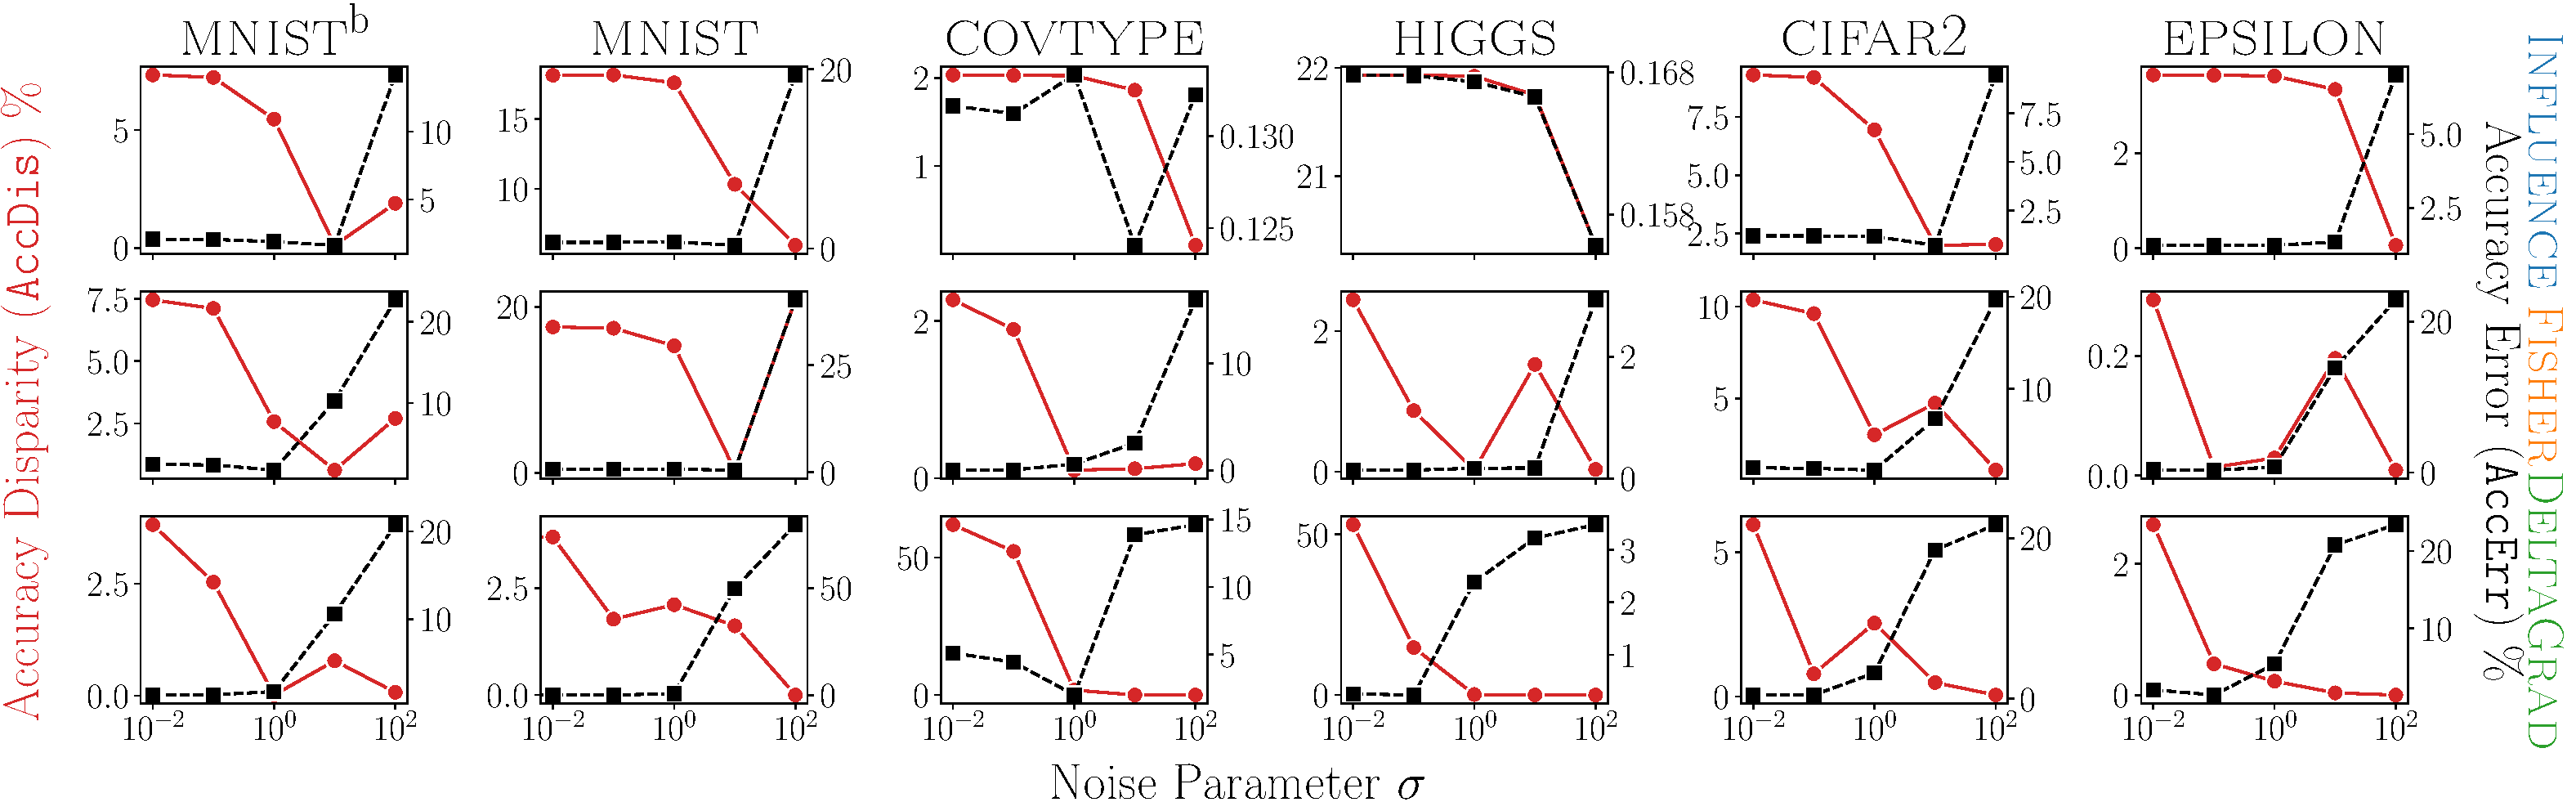
\includegraphics[width=0.5\linewidth,clip,trim={1.5cm 1cm 44cm 0 }]{./figs/Unlearning_Tradeoff_Grid.pdf}
%                 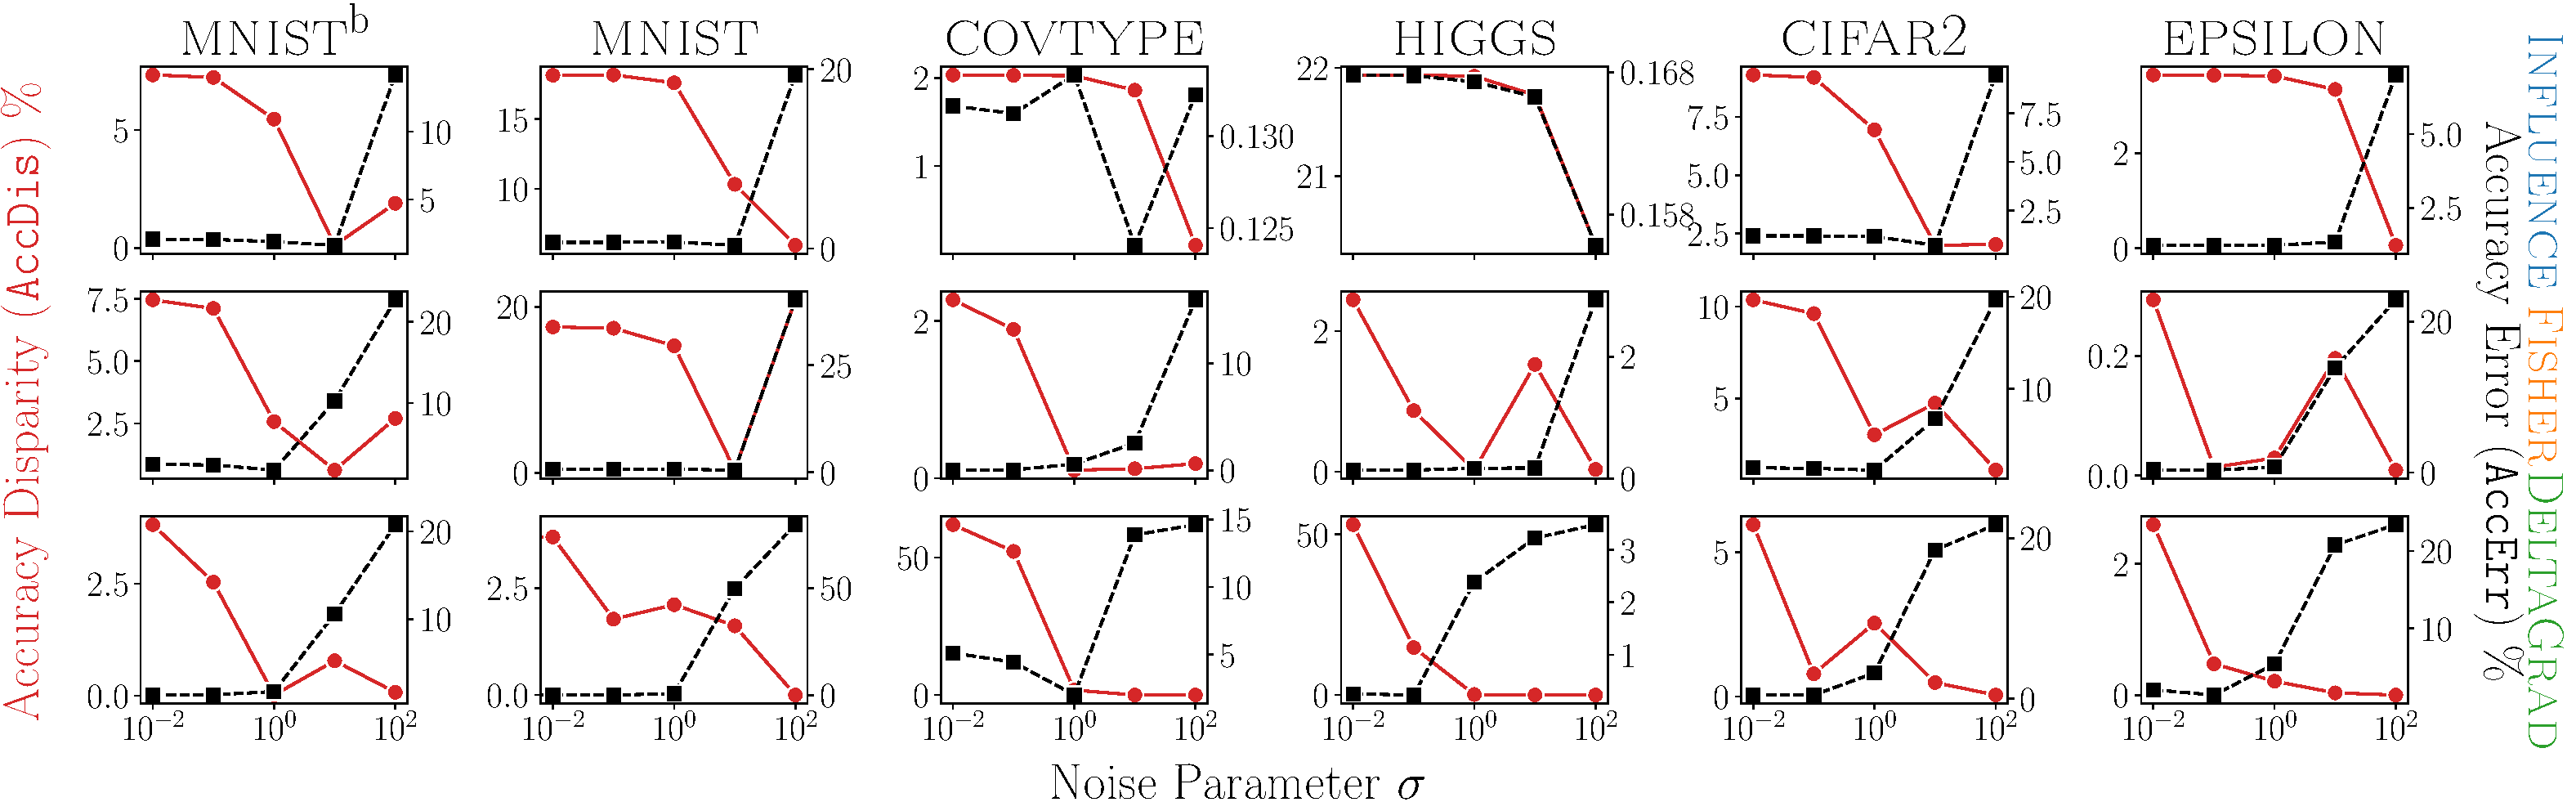
\includegraphics[width=0.13\linewidth,clip,trim={51.3cm 0.8cm 0 0 }]{./figs/Unlearning_Tradeoff_Grid.pdf}\\
%                 {\small Noise Paramter \noiseParamter}
%             \end{center}
%         \end{column}
%     \end{columns}
        
% \end{frame}

% \begin{frame}
%     \frametitle{Employ or Retrain}
%     \begin{itemize}
%         \item Multiple unlearning stages decrease certifiability
%         \item Retraining restarts pipeline \& resets certifiability
%         \item How to estimate certifiability?
%         \item When to trigger retraining? 
%       \end{itemize}
%       \begin{center}
%         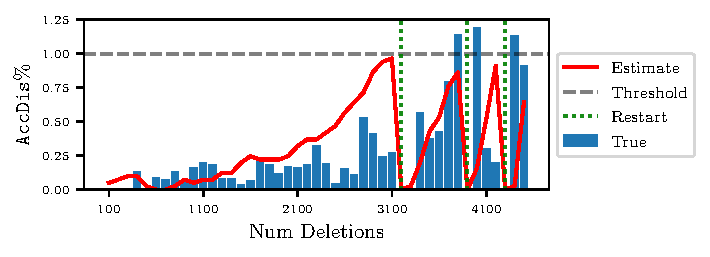
\includegraphics[width=\linewidth,clip,trim={ 2.5mm 0 2mm 0}]{./figs/MNIST_binary_targeted_informed_threshold_1_acc_dis_noise_1.pdf}
%       \end{center}
  

% \end{frame}
\againframe<2>{published}


\begin{frame}
    \frametitle{Scaling Node Classification \cite{merchant2022JANE}}
    \begin{figure}
        \centering
        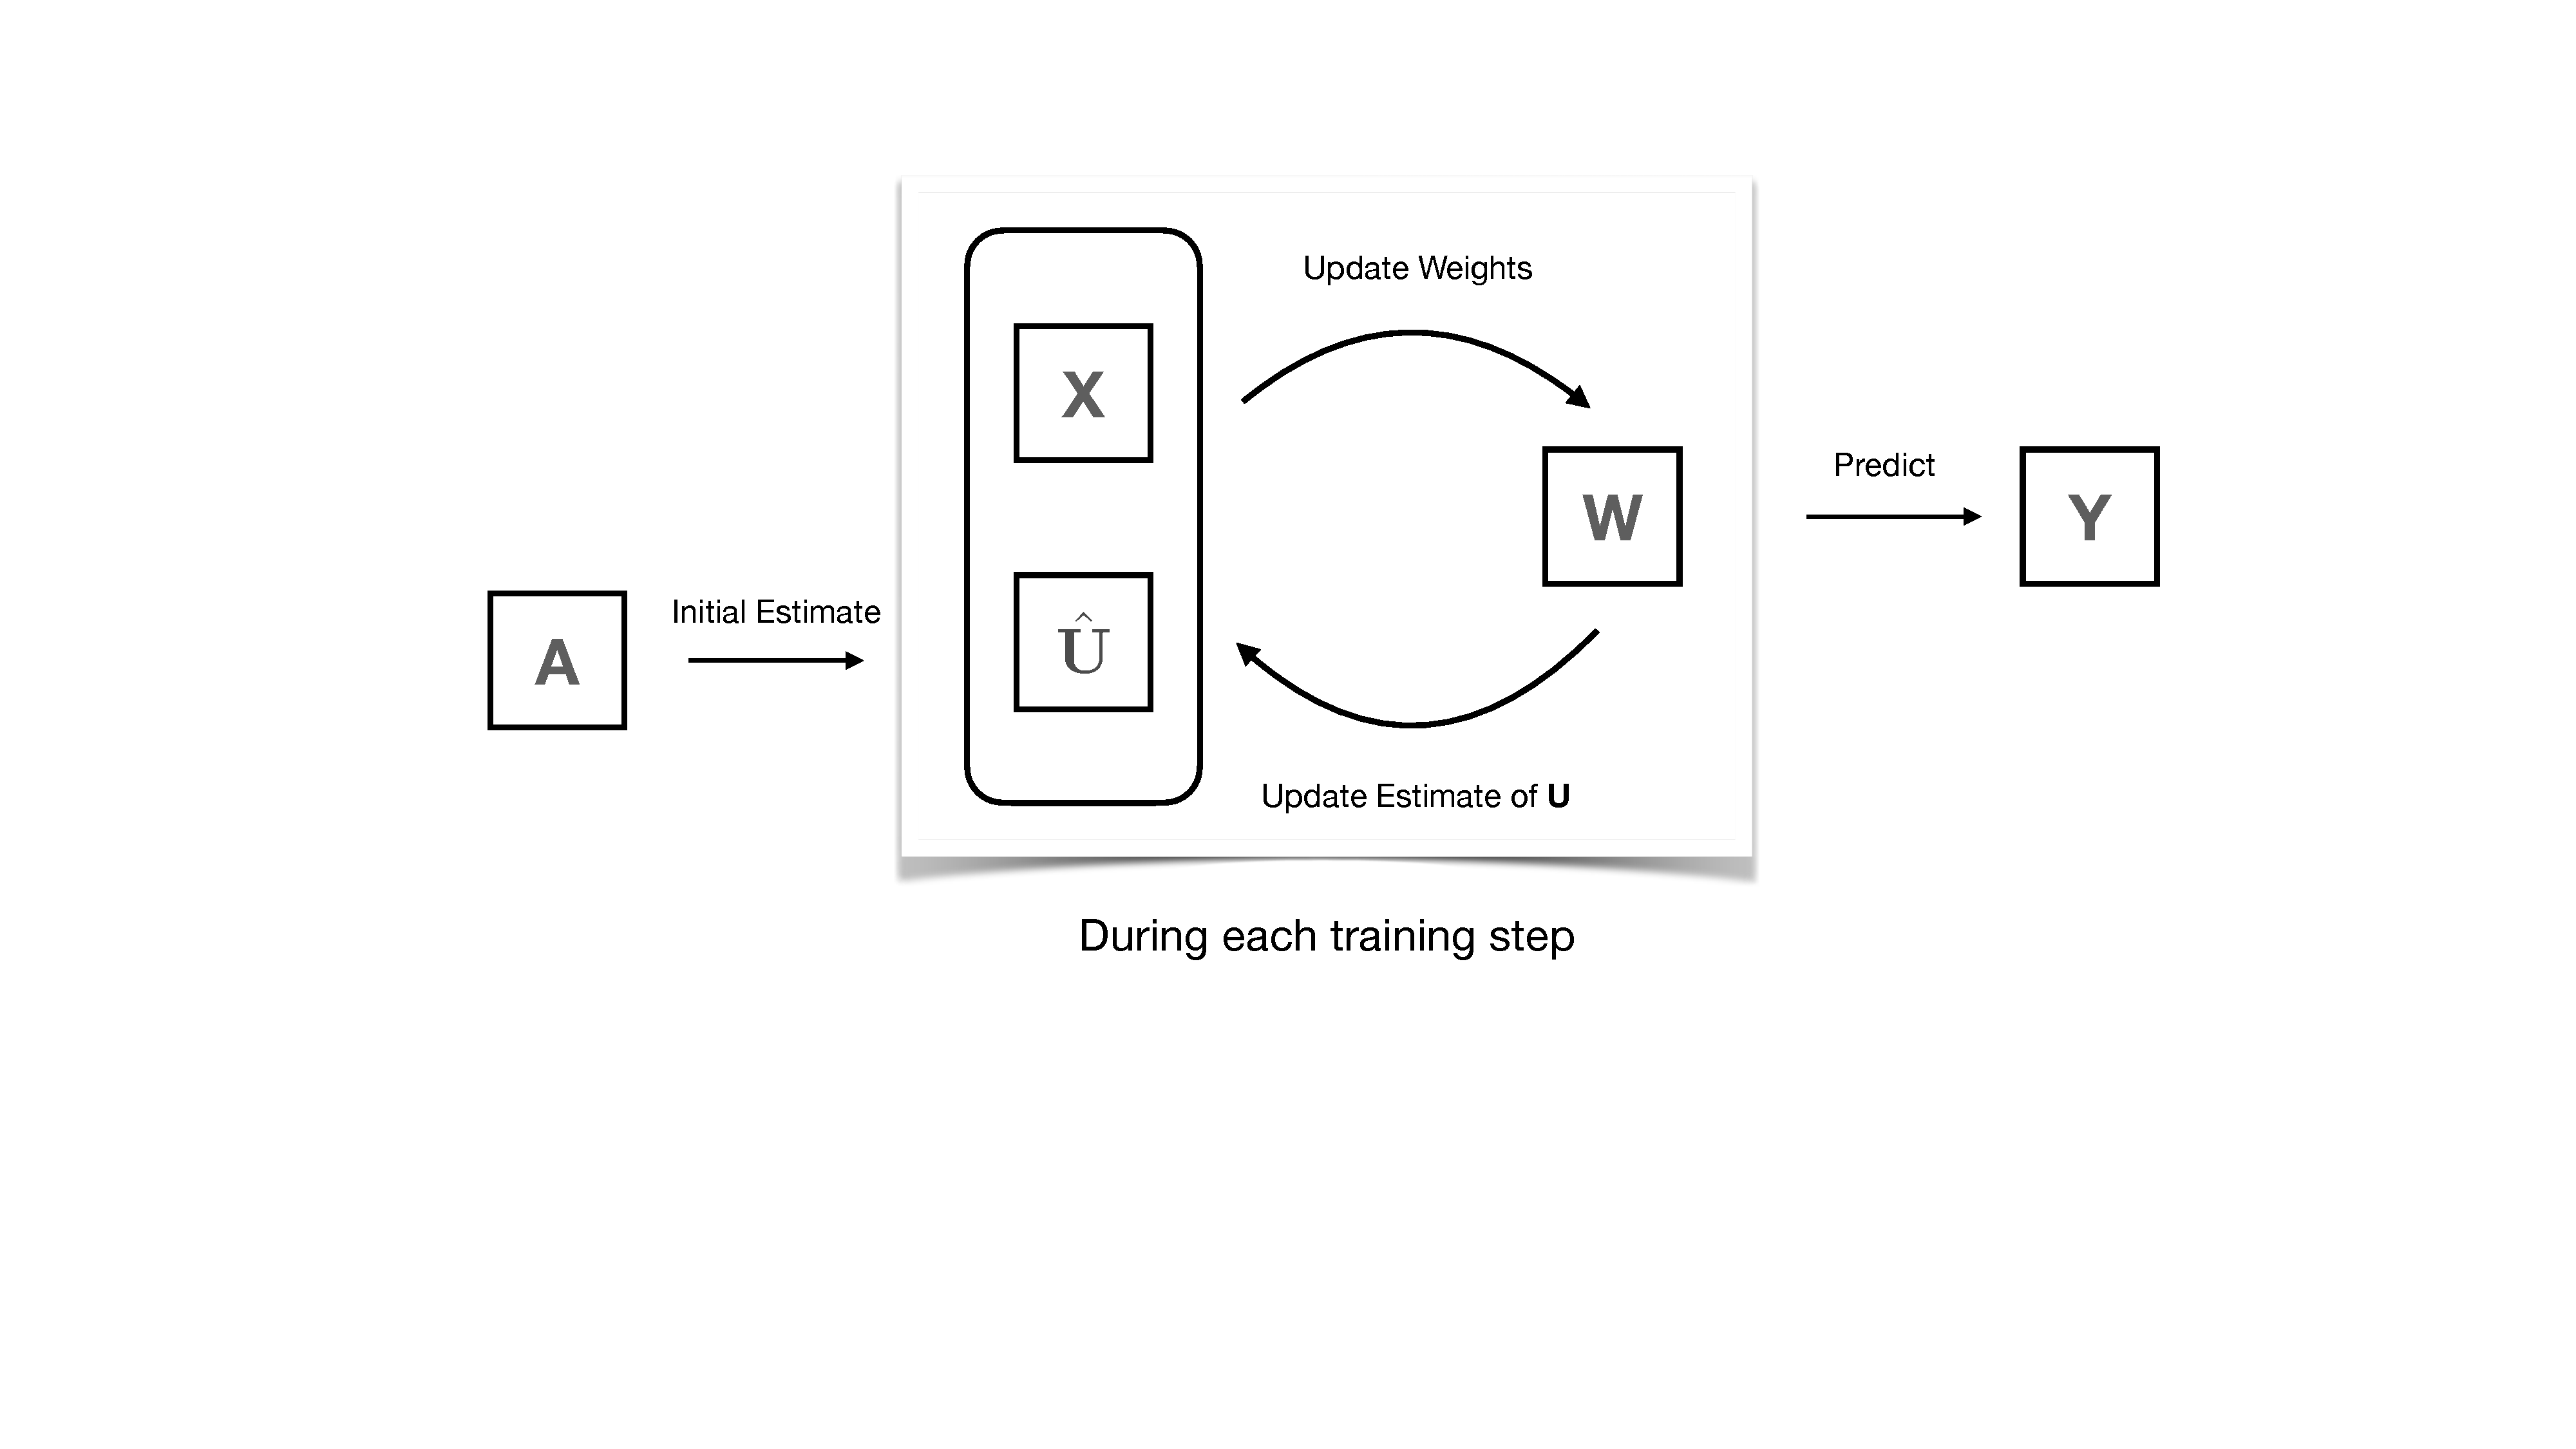
\includegraphics[width=0.5\textwidth]{figs/JANE.pdf}
    \end{figure}
    \begin{itemize}
        \item Improves running time of node classification method JANE \cite{merchant2022JANEorig}
        \item Developed mini-batching training algorithm to improve GPU utilization
        \item Scaled experiments to graphs with more than a million nodes
    \end{itemize}

\end{frame}
    
\againframe<3>{published}

\begin{frame}
    \frametitle{Robustness of Sketched Linear Classifiers \cite{mahadevan2022certifiable}}
    \begin{columns}
        \begin{column}{0.4\textwidth}
           \begin{itemize}
            \item \w: Linear Classifier
            \item \z: \wmsketch Classifier \cite{tai2018sketch}
            \item \adv: Adversary
            \item \perturb: FGSM perturbation
           \end{itemize}
        \end{column}
        \begin{column}{0.6\textwidth}
            \begin{center}
                \scalebox{0.85}{
                \begin{tikzpicture}
                    \begin{scope}
    % positioning style from https://tex.stackexchange.com/questions/102250/how-to-position-one-node-relative-to-another-node-at-a-certain-angle-in-tikz-tak
\tikzset{
        position/.style args={#1:#2 from #3}{
            at=(#3.#1), anchor=#1+180, shift=(#1:#2)
        }
    }

% database shape from from https://tex.stackexchange.com/questions/442991/database-shape-in-tikz
\tikzset{class1/.style={rectangle,thick,draw, inner sep=1mm, outer sep=0mm,fill=red}}
\tikzset{class2/.style={circle,draw,thick,inner sep=1mm, outer sep=0mm,fill=blue!60}}


\begin{scope}

    % helpers, comment them out in the final 
    % \draw[help lines] (-1,-4) grid (4,2);
    % \node[draw,circle] (origin) at (0,0) {};

    % https://tex.stackexchange.com/questions/245657/how-can-i-randomly-perturb-the-position-of-a-grid-of-nodes
    % \pgfmathsetseed{3} 
    % \foreach \i in {0,2,...,4}
    % \foreach \j in {0,2,...,4}
    %     {   
    %         draw grid
    %         \node [class1,fill=none] (g1-\i\j) at (\i/2,\j/2) {};
    %         perturb grid points
    %         \node [class1,fill=red!40] (n1-\i\j) at (\i/2 + 0.5*rand,\j/2 + 0.5*rand) {};
    %         \node [class1,fill=white,opacity=0.1] (n1-\i\j) at (\i/2,\j/2 ) {};
    %         }
    \node [class1] (n1-00) at (-0.3,0.2) {};
    \node [class1] (n1-02) at (0.34,0.8) {};
    \node [class1] (n1-04) at (-0.6,1.7) {};
    \node [class1] (n1-20) at (0.7,0) {};
    \node [class1] (n1-22) at (1.7,1.25) {};
    \node [class1] (n1-24) at (0.65,1.6) {};
    \node [class1] (n1-40) at (1.2,0.7) {};
    \node [class1] (n1-42) at (2.2,0.6) {};
    \node [class1] (n1-44) at (1.25,2) {};
    
    % \foreach \i in {0,2,...,4}
    % \foreach \j in {0,2,...,4}
    % {           
    %     %draw grid  
    %     % \node [class1,fill=none] (g2-\i\j) at (\i/2+2.5,\j/2-3) {};
    %     % perturb grid points
    %     % \node [class2] (n2-\i\j) at (2.5+\i/2 + 0.25*rand,\j/2 + 0.25*rand - 3) {};
    %     \node [class2,fill=white,opacity=0.1] (n2-\i\j) at (2.5+\i/2,\j/2 - 3) {};
    %     }
    \node [class2] (n2-00) at (2.5,-3) {};
    \node [class2] (n2-02) at (2.5+0.34,0.8-3) {};
    \node [class2] (n2-04) at (2.5+-0.6,1.7-3) {};
    \node [class2] (n2-20) at (2.5+1,-0.5-3) {};
    \node [class2] (n2-22) at (2.5+1.7,1.25-3) {};
    \node [class2] (n2-24) at (2.5+0.65,1.6-3) {};
    \node [class2] (n2-40) at (2.5+1.4,0.4-3) {};
    \node [class2] (n2-42) at (2.5+2.2,0.6-3) {};
    \node [class2] (n2-44) at (2.5+1.25,2-3) {};
    % \node[rectangle,draw=none,minimum size=30mm] at (-2,-0.5) {};
    % \draw[white] (-1,-2) -- (5,0) node[draw=none,above right] {};
\end{scope}
    \tikzset{pic/.style={inner sep=0mm,outer sep=0mm}}

\begin{scope}
    % positioning style from https://tex.stackexchange.com/questions/102250/how-to-position-one-node-relative-to-another-node-at-a-certain-angle-in-tikz-tak
\tikzset{
        position/.style args={#1:#2 from #3}{
            at=(#3.#1), anchor=#1+180, shift=(#1:#2)
        }
    }

% database shape from from https://tex.stackexchange.com/questions/442991/database-shape-in-tikz
\tikzset{class1/.style={rectangle,thick,draw, inner sep=1mm, outer sep=0mm,fill=red}}
\tikzset{class2/.style={circle,draw,thick,inner sep=1mm, outer sep=0mm,fill=blue!60}}


\begin{scope}

    % helpers, comment them out in the final 
    % \draw[help lines] (-1,-4) grid (4,2);
    % \node[draw,circle] (origin) at (0,0) {};

    % https://tex.stackexchange.com/questions/245657/how-can-i-randomly-perturb-the-position-of-a-grid-of-nodes
    % \pgfmathsetseed{3} 
    % \foreach \i in {0,2,...,4}
    % \foreach \j in {0,2,...,4}
    %     {   
    %         draw grid
    %         \node [class1,fill=none] (g1-\i\j) at (\i/2,\j/2) {};
    %         perturb grid points
    %         \node [class1,fill=red!40] (n1-\i\j) at (\i/2 + 0.5*rand,\j/2 + 0.5*rand) {};
    %         \node [class1,fill=white,opacity=0.1] (n1-\i\j) at (\i/2,\j/2 ) {};
    %         }
    \node [class1] (n1-00) at (-0.3,0.2) {};
    \node [class1] (n1-02) at (0.34,0.8) {};
    \node [class1] (n1-04) at (-0.6,1.7) {};
    \node [class1] (n1-20) at (0.7,0) {};
    \node [class1] (n1-22) at (1.7,1.25) {};
    \node [class1] (n1-24) at (0.65,1.6) {};
    \node [class1] (n1-40) at (1.2,0.7) {};
    \node [class1] (n1-42) at (2.2,0.6) {};
    \node [class1] (n1-44) at (1.25,2) {};
    
    % \foreach \i in {0,2,...,4}
    % \foreach \j in {0,2,...,4}
    % {           
    %     %draw grid  
    %     % \node [class1,fill=none] (g2-\i\j) at (\i/2+2.5,\j/2-3) {};
    %     % perturb grid points
    %     % \node [class2] (n2-\i\j) at (2.5+\i/2 + 0.25*rand,\j/2 + 0.25*rand - 3) {};
    %     \node [class2,fill=white,opacity=0.1] (n2-\i\j) at (2.5+\i/2,\j/2 - 3) {};
    %     }
    \node [class2] (n2-00) at (2.5,-3) {};
    \node [class2] (n2-02) at (2.5+0.34,0.8-3) {};
    \node [class2] (n2-04) at (2.5+-0.6,1.7-3) {};
    \node [class2] (n2-20) at (2.5+1,-0.5-3) {};
    \node [class2] (n2-22) at (2.5+1.7,1.25-3) {};
    \node [class2] (n2-24) at (2.5+0.65,1.6-3) {};
    \node [class2] (n2-40) at (2.5+1.4,0.4-3) {};
    \node [class2] (n2-42) at (2.5+2.2,0.6-3) {};
    \node [class2] (n2-44) at (2.5+1.25,2-3) {};
    % \node[rectangle,draw=none,minimum size=30mm] at (-2,-0.5) {};
    % \draw[white] (-1,-2) -- (5,0) node[draw=none,above right] {};
\end{scope}
    \draw[very thick] (-0.5,-4) -- (3.5,2) node[left] {\w};
    
    \node[pic] (orig3) at (-0.5,-1) {
\includegraphics[width=0.1\textwidth]{figs/orig_3.pdf}};
    
    \node[pic] (orig7) at (1.2,-3) {
\includegraphics[width=0.1\textwidth]{figs/orig_7.pdf}};
    
    \draw[-,thick] (n1-20.north west) -- (orig3.north west);
    \draw[-,thick] (n1-20.south east) -- (orig3.south east);
    
    \draw[-,thick] (n2-02.120) -- (orig7.north west);
    \draw[-,thick] (n2-02.300) -- (orig7.south east);
\end{scope}
    \node[class2,outer sep=0.2mm,draw=red,very thick] (adv) at (2.5,-0.5) {};
    \node[devil,blackbox,minimum size=5mm] at (-1,0.5) {\adv};
    \draw[
        -,dashed,thick,green!50!black,
        decoration={markings,mark=at position 0.5 with {\arrow{latex}}},
        postaction={decorate}
        ] 
        (n1-20) -- (adv) node[pos=0.5,above] {$\perturb > 0$};
    \node[pic] (white-box3) at (3.5,0.5) {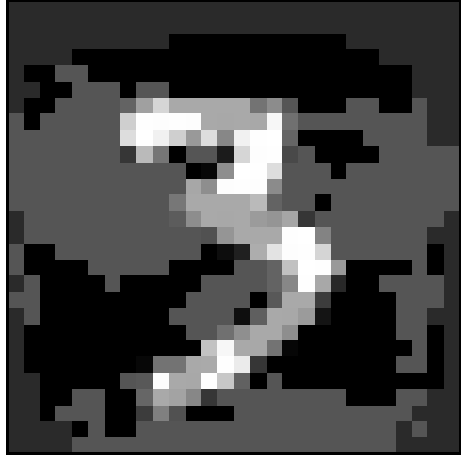
\includegraphics[width=0.1\textwidth]{figs/3_3.pdf}};
    \draw[-,thick] (adv.140) -- (white-box3.north west);
    \draw[-,thick] (adv.270) -- (white-box3.south east);
\end{scope}
                    \begin{scope}
    \tikzset{pic/.style={inner sep=0mm,outer sep=0mm}}

\begin{scope}
    % positioning style from https://tex.stackexchange.com/questions/102250/how-to-position-one-node-relative-to-another-node-at-a-certain-angle-in-tikz-tak
\tikzset{
        position/.style args={#1:#2 from #3}{
            at=(#3.#1), anchor=#1+180, shift=(#1:#2)
        }
    }

% database shape from from https://tex.stackexchange.com/questions/442991/database-shape-in-tikz
\tikzset{class1/.style={rectangle,thick,draw, inner sep=1mm, outer sep=0mm,fill=red}}
\tikzset{class2/.style={circle,draw,thick,inner sep=1mm, outer sep=0mm,fill=blue!60}}


\begin{scope}

    % helpers, comment them out in the final 
    % \draw[help lines] (-1,-4) grid (4,2);
    % \node[draw,circle] (origin) at (0,0) {};

    % https://tex.stackexchange.com/questions/245657/how-can-i-randomly-perturb-the-position-of-a-grid-of-nodes
    % \pgfmathsetseed{3} 
    % \foreach \i in {0,2,...,4}
    % \foreach \j in {0,2,...,4}
    %     {   
    %         draw grid
    %         \node [class1,fill=none] (g1-\i\j) at (\i/2,\j/2) {};
    %         perturb grid points
    %         \node [class1,fill=red!40] (n1-\i\j) at (\i/2 + 0.5*rand,\j/2 + 0.5*rand) {};
    %         \node [class1,fill=white,opacity=0.1] (n1-\i\j) at (\i/2,\j/2 ) {};
    %         }
    \node [class1] (n1-00) at (-0.3,0.2) {};
    \node [class1] (n1-02) at (0.34,0.8) {};
    \node [class1] (n1-04) at (-0.6,1.7) {};
    \node [class1] (n1-20) at (0.7,0) {};
    \node [class1] (n1-22) at (1.7,1.25) {};
    \node [class1] (n1-24) at (0.65,1.6) {};
    \node [class1] (n1-40) at (1.2,0.7) {};
    \node [class1] (n1-42) at (2.2,0.6) {};
    \node [class1] (n1-44) at (1.25,2) {};
    
    % \foreach \i in {0,2,...,4}
    % \foreach \j in {0,2,...,4}
    % {           
    %     %draw grid  
    %     % \node [class1,fill=none] (g2-\i\j) at (\i/2+2.5,\j/2-3) {};
    %     % perturb grid points
    %     % \node [class2] (n2-\i\j) at (2.5+\i/2 + 0.25*rand,\j/2 + 0.25*rand - 3) {};
    %     \node [class2,fill=white,opacity=0.1] (n2-\i\j) at (2.5+\i/2,\j/2 - 3) {};
    %     }
    \node [class2] (n2-00) at (2.5,-3) {};
    \node [class2] (n2-02) at (2.5+0.34,0.8-3) {};
    \node [class2] (n2-04) at (2.5+-0.6,1.7-3) {};
    \node [class2] (n2-20) at (2.5+1,-0.5-3) {};
    \node [class2] (n2-22) at (2.5+1.7,1.25-3) {};
    \node [class2] (n2-24) at (2.5+0.65,1.6-3) {};
    \node [class2] (n2-40) at (2.5+1.4,0.4-3) {};
    \node [class2] (n2-42) at (2.5+2.2,0.6-3) {};
    \node [class2] (n2-44) at (2.5+1.25,2-3) {};
    % \node[rectangle,draw=none,minimum size=30mm] at (-2,-0.5) {};
    % \draw[white] (-1,-2) -- (5,0) node[draw=none,above right] {};
\end{scope}
    \draw[very thick] (-0.5,-4) -- (3.5,2) node[left] {\w};
    
    \node[pic] (orig3) at (-0.5,-1) {
\includegraphics[width=0.1\textwidth]{figs/orig_3.pdf}};
    
    \node[pic] (orig7) at (1.2,-3) {
\includegraphics[width=0.1\textwidth]{figs/orig_7.pdf}};
    
    \draw[-,thick] (n1-20.north west) -- (orig3.north west);
    \draw[-,thick] (n1-20.south east) -- (orig3.south east);
    
    \draw[-,thick] (n2-02.120) -- (orig7.north west);
    \draw[-,thick] (n2-02.300) -- (orig7.south east);
\end{scope}
    \draw[very thick, purple] (-1,-2) -- (5,0) node[above right] {\z};
\end{scope}
                  \end{tikzpicture}
                }
             \end{center}
        \end{column}
        \end{columns}

\end{frame}


\begin{frame}
    \frametitle{Robustness of Sketched Linear Classifiers \cite{mahadevan2022certifiable}}
    \adv crafts a perturbation based on its Knowledge and Observability of the target.
    \begin{itemize}
      \item \textcolor{blue!80}{Knowledge}: Is the target a \wmsketch?
      \item \textcolor{blue!80}{Observability}: Does \adv have access to count sketch \JLmat?
    \end{itemize}
    \begin{center}
    \begin{tabular}{c|c|c}
      \toprule
      \adv      & Knowledge & Observability \\
      \midrule
      White-Box & \cmark    & \cmark        \\
      Grey-Box  & \cmark    & \xmark        \\
      Black-Box & \xmark    & \xmark        \\
      \bottomrule
    \end{tabular}
  \end{center}
  \begin{block}{Research Question}
    How does the performance of a given \textnormal{\wmsketch} worsen in the presence of these adversaries?
  \end{block}

\end{frame}

\againframe<4>{published}

\begin{frame}
    \frametitle{Reception Reader Interface}
    \begin{figure}[htbp]
        \centering
        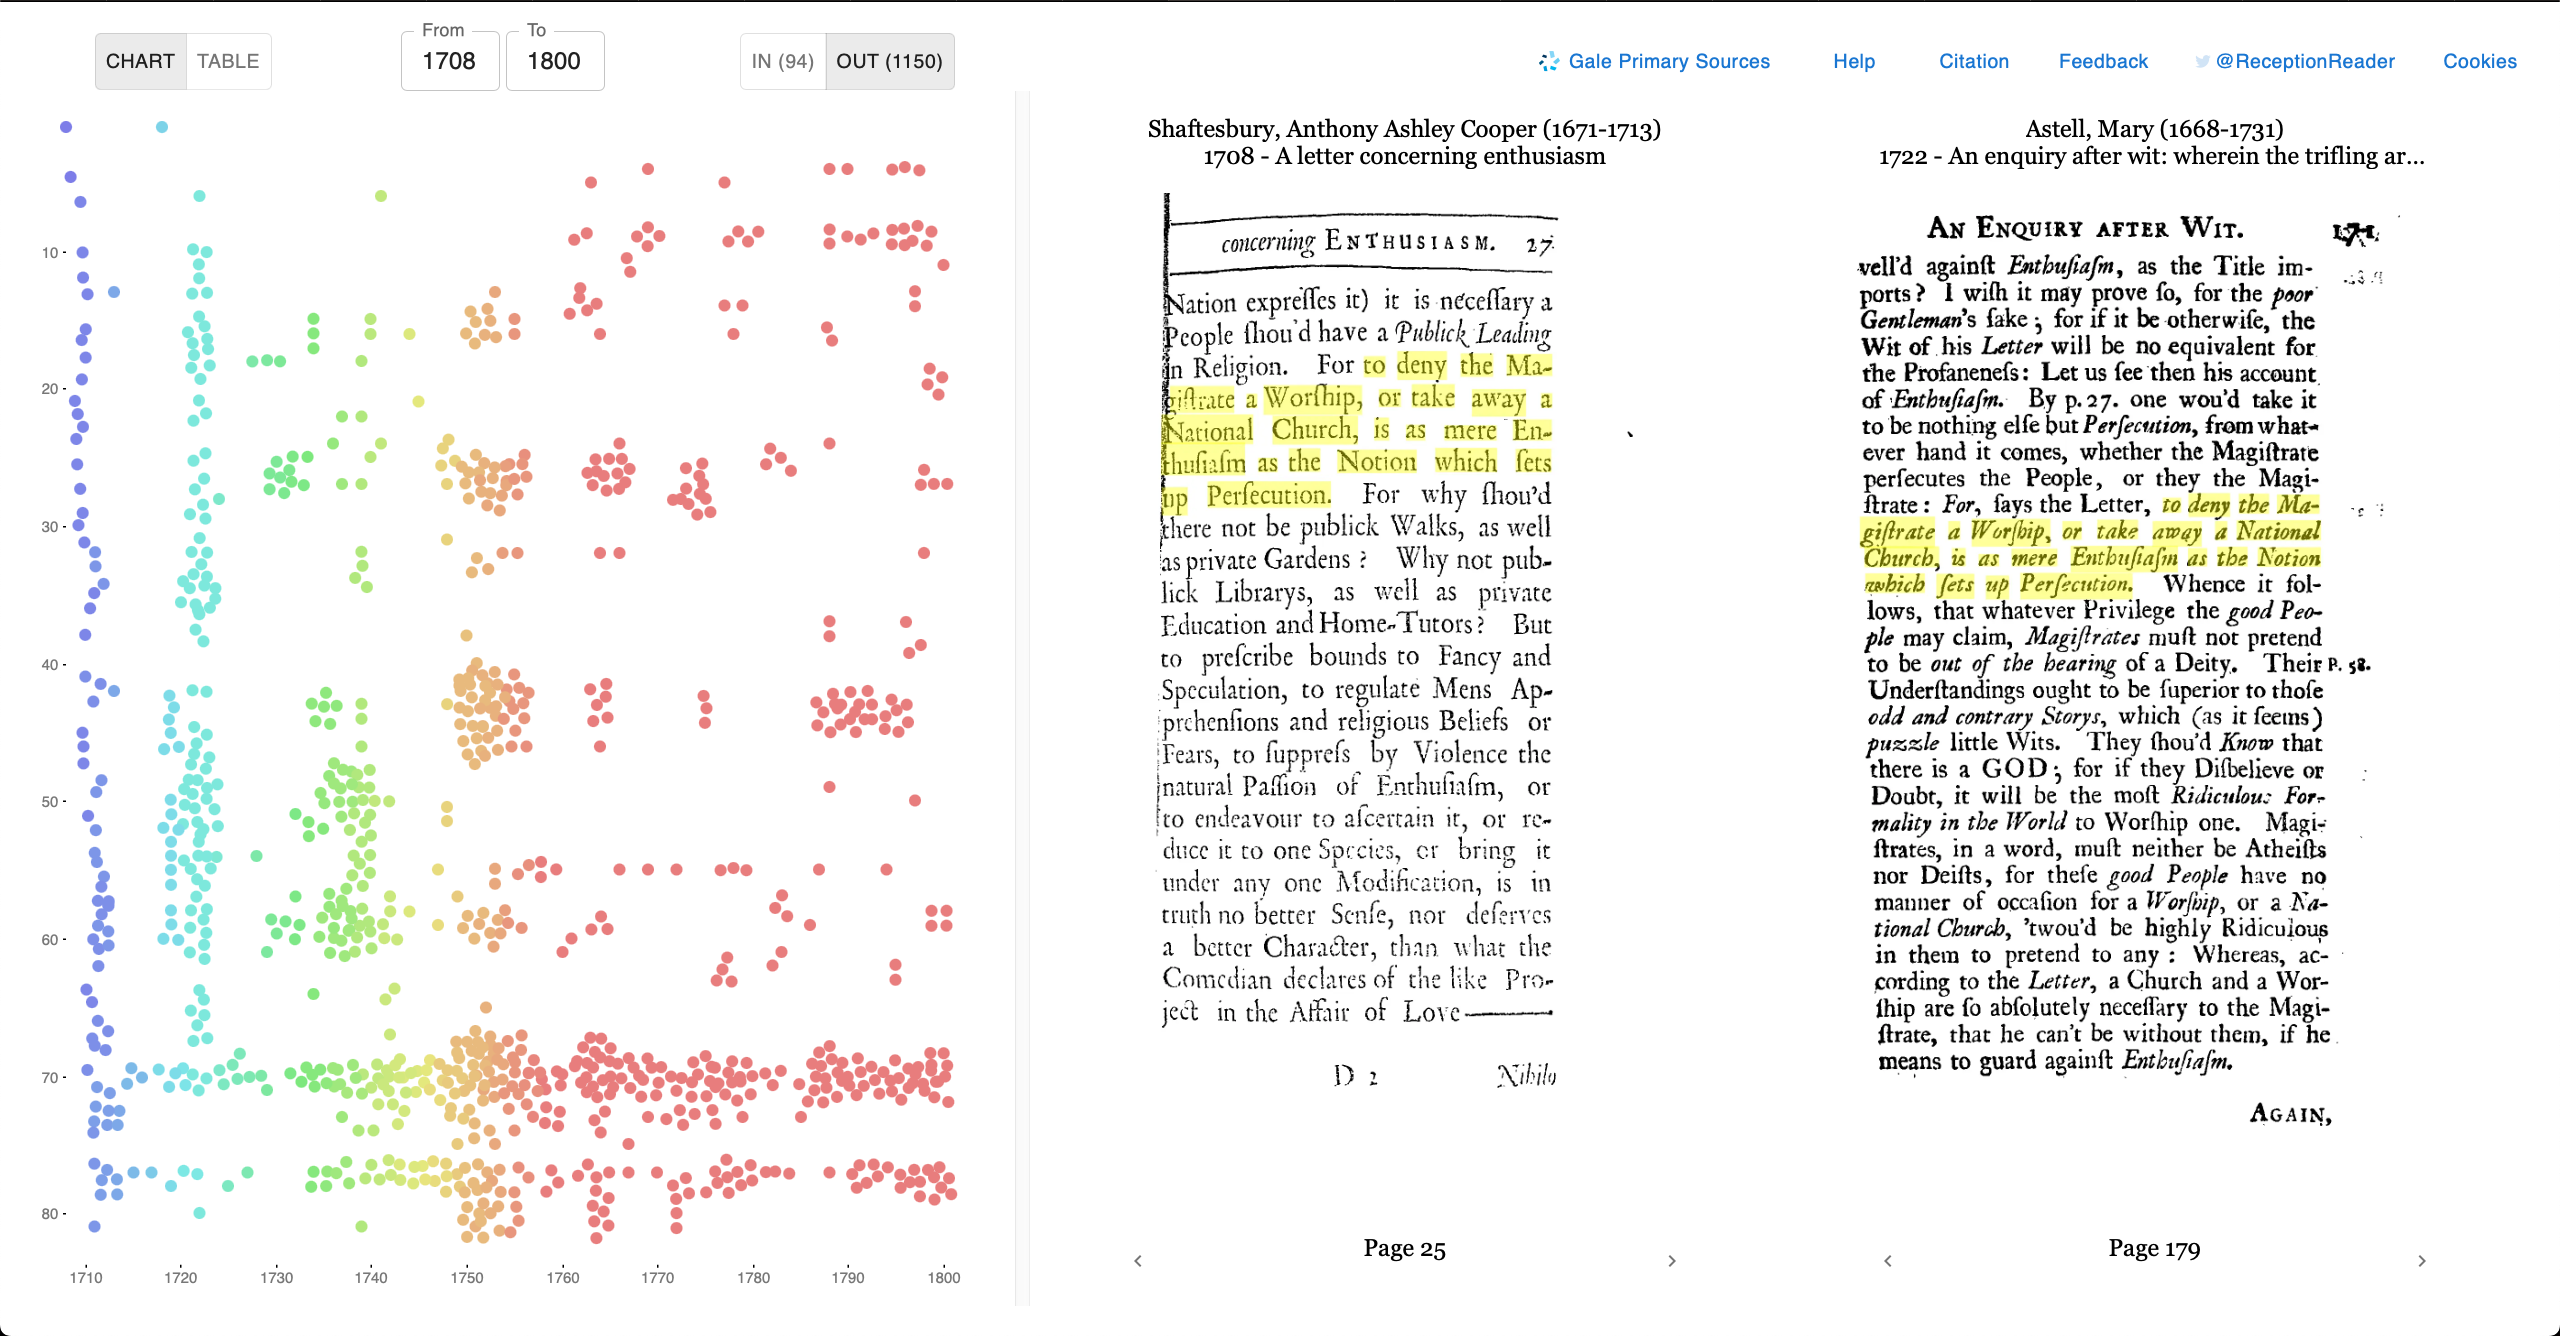
\includegraphics[width=\textwidth]{figs/Reception Reader.png}
    \end{figure}
\end{frame}

\begin{frame}
    \frametitle{Historical Text Reuse}

    \begin{itemize}
        \item 250k scanned English documents from 18th century
        \item Fuzzy string matching using BLAST to find reuses
        \item De-fragmenting and clustering of reuse pairs
        \item Front-end for navigation
    \end{itemize}

\end{frame}


\subsection{Works in Progress}
\begin{frame}<1>[label=progress]
    \frametitle{In Progress}
    \begin{enumerate}[<+->]
        \item Cost-Aware Retraining for Machine Learning
        \begin{itemize}[<.->]
            \item Rejections from ICML 2023 and EuroSys 2023
            \item Submitted pre-print to Arxiv \cite{mahadevan2023costeffective}
            \item Re-submitted to Knowledge-Based Systems Journal
        \end{itemize}
        \item Data Science Pipeline for Historical Text Reuse
        \begin{itemize}[<.->]
            \item Manuscript under preparation
            \item Planned submission to VLDB 2024 Scalable Data Science track
        \end{itemize}
        \item Scalable Constraint-Based Diversity Sampling
        \begin{itemize}[<.->]
            \item Improved running time of Fair Max-Min Diversification \citep{wang2023fmmd}
            \item Plan to develop approximate distributed sampling algorithm and code library
        \end{itemize}
    \end{enumerate}

\end{frame}


\begin{frame}
    \frametitle{Cost-Aware Retraining for ML}
    \begin{figure}[h]
        \centering
        {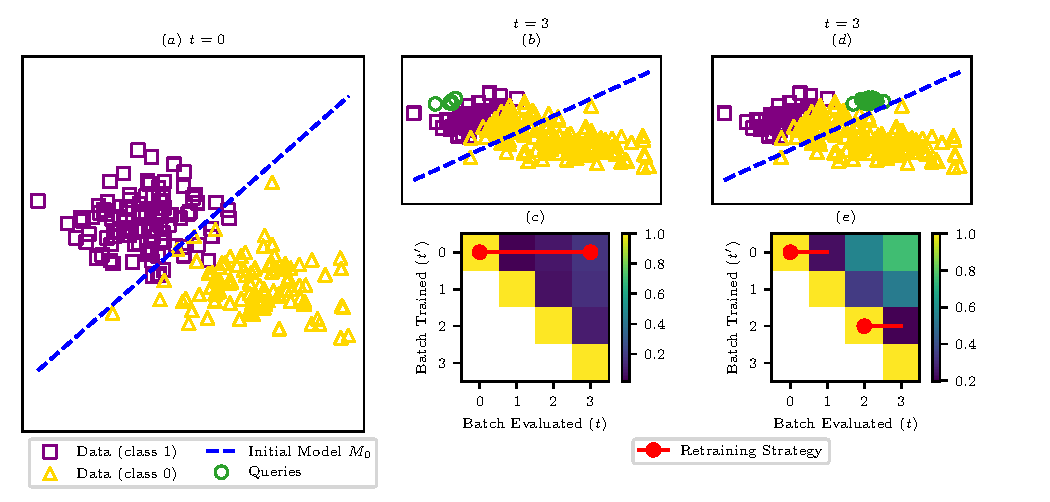
\includegraphics[width=0.8\textwidth,clip,trim={0 2.5mm 0 5.5mm}]{figs/proof_of_concept.pdf}}
        \caption{Example scenario. (a) Initial data and model $\model_0$. (b) Queries are far from misclassification. (d) Queries are closer to misclassifications. (c) and (e): Cost matrix and \oracle retraining strategies with retraining cost fixed to $\retraincost=1$ for (b) and (d) respectively.}
        \label{fig:scenario-1-extended}
    \end{figure}
    

\end{frame}


\againframe<2>{progress}

\begin{frame}
    \frametitle{Dagster ETL pipeline}
    \begin{figure}
        \centering
        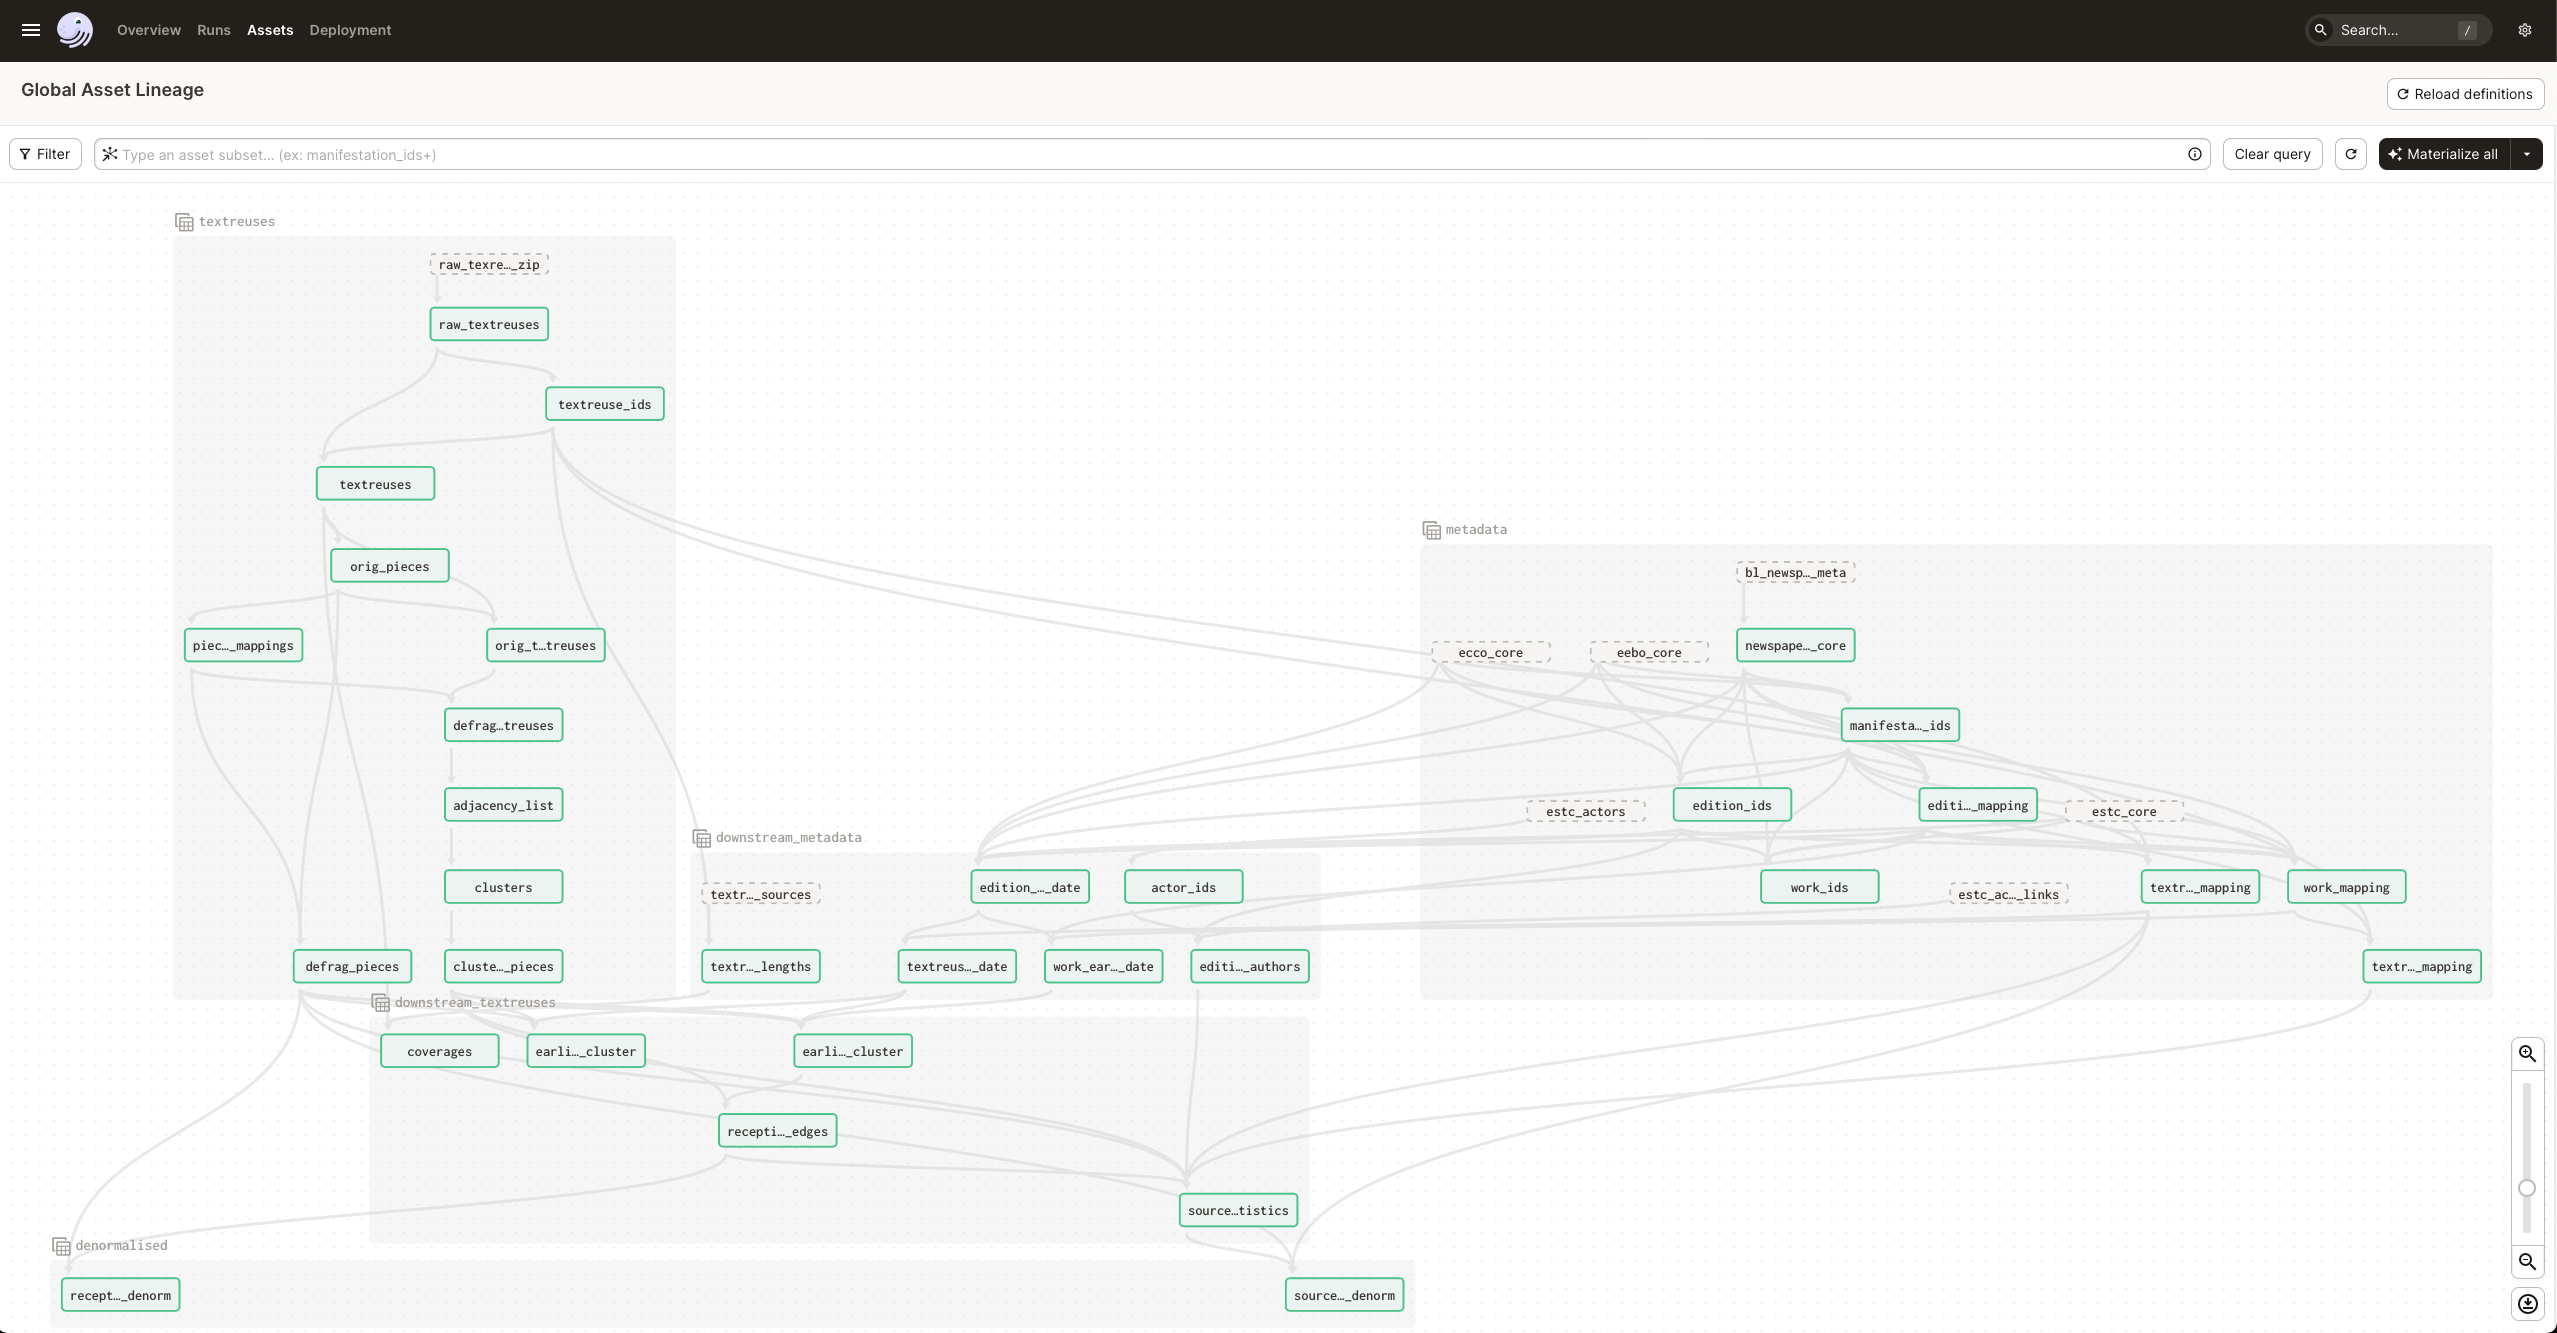
\includegraphics[width=\textwidth]{figs/dagster.png}
        
    \end{figure}
    

\end{frame}

\begin{frame}
    \frametitle{Experiments}
    \begin{itemize}
        \item Benchmarking query performance on
        \begin{enumerate}
            \item Spark
            \item MariaDB Aria
            \item MariaDB Columnstore
        \end{enumerate}
        \item Evaluating different metrics
        \begin{enumerate}
            \item Query Latency
            \item Storage size
            \item Cost in CSC BU    
        \end{enumerate}
        \item Different levels of normalisation 
    \end{itemize}
    

\end{frame}


\againframe<3>{progress}

\begin{frame}
    \frametitle{Scaling up Fair-MMD}
    Completed
    \begin{itemize}
        \item Reimplementation of FMMD-S algorithm from \cite{wang2023fmmd}
        \item Parallelizes sections of code and efficient memory management
        \item $100\times$ speedup on largest experiment from \cite{wang2023fmmd}
        \item Scaled up to 4M points dataset and 3000 samples with edge-case constraints
    \end{itemize}
    Next Steps
    \begin{itemize}
        \item Distributed algorithm with gurantees
        \item Approximate distance measures
        \item Heuristic based ILP solver
    \end{itemize}
\end{frame}

\section{Studies}

\subsection{Discipline Specific Credits}
\begin{frame}
    \frametitle{Discipline Specific Credits}

    \begin{block}{Completed Credits}
        $29/30$ credits completed excluding PhD Seminar (3-5 credits)
    \end{block}
    Completed Courses:
    \begin{itemize}
        \item Network Analysis 5cr
        \item Security and Privacy in ML 5cr
        \item Advanced Latex Course 5cr
        \item Probabilistic Graphical Models 5cr
        \item Advanced Course in Machine Learning 5cr 
        \item Transaction Management and Query Optimization 5cr
        \item Research Ethics 2 cr
    \end{itemize}
\end{frame}

\subsection{Transferrable Skills}

\begin{frame}
    \frametitle{Transferrable Skills}
    Completed Courses 3cr:
    \begin{itemize}
        \item Scientific Writing 2cr 
        \item Principles of Peer Review 1cr
    \end{itemize}
    Planned Credits 7cr:
    \begin{itemize}
        \item Conference Presentation 2cr   
        \item Poster Presentation and Data Visualization 2cr
        \item International Conference participation 2cr
        \item Grant Writing 1cr
    \end{itemize}

\end{frame}

\section{Activities}

\subsection{Conferences, Workshops and Events}
\begin{frame}
    \frametitle{Conferences}
    \begin{itemize}
        \item VLDB 2022: Participation
        \item CIKM 2022: Presentation (virtual)
        \item MLSys 2023: Participation
        \item AI Day 2022: Poster Presentation
        \item Meaning of Meaning Workshop 2023: Presentation
    \end{itemize}

    
\end{frame}

\subsection{Teaching and Supervision}
\begin{frame}
    \frametitle{Teaching and Supervision}

    \begin{itemize}
        \item  TA: Netowork Analysis 2023
        \item Master Thesis Instruction: Anniina R Sainio (Completed)
        \item Master Thesis Instruction: Andreas Maniatas (Ongoing)
    \end{itemize}
\end{frame}

\section{Future Plans}


\begin{frame}
    \frametitle{Plans for 2023-2024}
    \begin{enumerate}
        \item Research
        \begin{itemize}
            \item Present - Nov 2023: Submit ``Data Science Pipeline for Historical Text Reuse'' to VLDB
            \item Jan - Mar 2024: Complete scalable sampling project
        \end{itemize}
        \item Studies
        \begin{itemize}
            \item Complete remaining transferrable course credits
            \item Finalize all credits with Pirio
        \end{itemize}
        \item Thesis
        \begin{itemize}
            \item Mar 2024 - May 2024: Thesis Writing
            \item June 2024: Pre-examination
        \end{itemize}
    \end{enumerate}
    

\end{frame}

\begin{frame}[allowframebreaks]
    \frametitle{References}
    \bibliographystyle{plain}
    \bibliography{references}
  \end{frame}


\begin{frame}
    \frametitle{Thesis inclusion of works}
    Minimum Works in Thesis
    \begin{enumerate}
        \item Certifiable Unlearning 
        \item Robustness of Sketched models
        \item Cost-Aware Retraining
        \item ETL pipeline for historical text reuse data
    \end{enumerate}
    Additional works 
    \begin{enumerate}
        \item Scaling up JANE 
        \item Scalable Diversity Sampling
        \item Reception Reader Interface
        \item Humanities Text Reuse use-case
    \end{enumerate}
    

\end{frame}

\begin{frame}
    \frametitle{Structure of Thesis}
    Tentative Organization of Works:
    \begin{enumerate}
        \item Maintaining ML models
        \begin{itemize}
            \item Certifiable Unlearning \cite{mahadevan2022certifiable}
            \item Cost-Aware Retraining \cite{mahadevan2023costeffective}
            \item Robustness of Sketched models \cite{10.1145/3511808.3557687}
        \end{itemize} 
        \item Scalable ML Pipelines
        \begin{itemize}
            \item JANE for node-classification \cite{merchant2022JANE}
            \item Scalable Diversity Sampling 
            \item Scalable Historical Text Reuse
            \begin{itemize}
                % \item Text Reuse dataset paper
                \item ETL pipeline paper 
                \item Reception Reader interface \cite{Rosson-2023}
                \item Humanities use-case paper
            \end{itemize}
        \end{itemize}
    \end{enumerate}
    

\end{frame}
\end{document}  